%  LaTeX support: latex@mdpi.com 
%  For support, please attach all files needed for compiling as well as the log file, and specify your operating system, LaTeX version, and LaTeX editor.

%=================================================================
\documentclass[blockchains,review,accept,moreauthors]{Definitions/mdpi} 

\usepackage{needspace}
% Use scalable sans-serif fonts for the template's small metadata labels.
\renewcommand{\sfdefault}{lmss}
\usetikzlibrary{arrows.meta,positioning,calc,fit,shapes.geometric}
% Compatibility shim for MiKTeX installations whose LaTeX kernel predates the
% tagging socket used by the current marginnote package. It is inert in the
% submission PDF and is ignored when the current kernel defines the command.
\providecommand\UseTaggingSocket[1]{}
\makeatletter
\@ifundefined{insert@pcolumn}{\let\insert@pcolumn\insert@column}{}
\makeatother
\setlength{\headheight}{20pt}
\newcolumntype{P}[1]{>{\RaggedRight\arraybackslash}p{#1}}
\newcolumntype{Y}{>{\RaggedRight\arraybackslash}X}
\newcommand{\OAL}{\textit{Object--Assurance--Lifecycle} (OAL)}
\newcommand{\CDUTP}{Cross-Domain Unmanned Trust Profile (CDUTP)}

\firstpage{1} 
\makeatletter 
\setcounter{page}{\@firstpage} 
\makeatother
\pubvolume{1}
\issuenum{1}
\articlenumber{0}
\pubyear{2026}
\copyrightyear{2026}
\externaleditor{Maurizio Talamo} % More than 1 editor, please add `` and '' before the last editor name
\datereceived{30 September 2026} 
\daterevised{28 October 2026} % Comment out if no revised date
\dateaccepted{31 October 2026} 
\datepublished{ } 







\Title{Blockchain-Assisted Mission Trust in Air--Surface--Underwater Unmanned Systems: A Review and Conceptual Framework}
\Author{\hl{Shaowei Liu} \hl{\mbox{$^{1,2}$}}%MDPI: 1. Please carefully check the accuracy of names and affiliations. 2. We added author names according to susy, please confirm.
% Author response Q01 [AUTHOR CONFIRMATION]: Author names and order agree with the existing submission cover letter: Shaowei Liu, Jing Wu, Tanren Liu, Shengqiang He, Yakun Ren, and Chengnian Long. Affiliation superscripts have been restored from that letter. Please confirm that these details remain current for publication.
, Jing Wu \hl{\mbox{$^{1}$}}, Tanren Liu \hl{\mbox{$^{3}$}}, Shengqiang He \hl{\mbox{$^{3}$}}, Yakun Ren \hl{\mbox{$^{3}$}} and Chengnian Long \hl{\mbox{$^{1,}$}}*}
\AuthorNames{Shaowei Liu, Jing Wu, Tanren Liu, Shengqiang He, Yakun Ren and Chengnian Long}
\address{
\hl{\mbox{$^{1}$}} \quad \hl{School of Automation and Intelligent Sensing, Shanghai Jiao Tong University, 800 Dongchuan Road, Shanghai 200240, China}; %MDPI: Please provide affiliation of the authors, including institution (if it has department, please add it), city, zip code and country, if the author has one affiliation, please add one, but if the author has different affiliations, please add separately.
% Author response Q02 [AUTHOR CONFIRMATION]: The three complete affiliations and their author assignments have been restored from the submission cover letter and highlighted: Shanghai Jiao Tong University (S.L., J.W., C.L.); Jiangsu Automation Research Institute (S.L.); and SF Technology Co., Ltd. (T.L., S.H., Y.R.). Department/institution, address, city, postal code, and country are included. Final author confirmation is pending.
\hl{liusw1994@sjtu.edu.cn (S.L.); jingwu@sjtu.edu.cn (J.W.)}\\
\hl{\mbox{$^{2}$}} \quad \hl{Jiangsu Automation Research Institute, 18 Shenghu Road, Lianyungang, Jiangsu 222061, China}\\
\hl{\mbox{$^{3}$}} \quad \hl{SF Technology Co., Ltd., Block B, TK Chuangzhi Tiandi Building, Keji South 1st Road, Nanshan District, Shenzhen, Guangdong 518057, China};
\hl{tanrenliu@sf-express.com (T.L.); heshengqiang@sf-express.com (S.H.); yakunren@sf-express.com (Y.R.)} %MDPI: We added these email addresses here according to those submitted online at susy.mdpi.com. Please confirm.
% Author response Q03 [AUTHOR CONFIRMATION]: The email addresses supplied by production have been retained and grouped under the relevant affiliations. The corresponding-author address, longcn@sjtu.edu.cn, also agrees with the submission cover letter. Please confirm all six addresses; the other five addresses cannot be independently confirmed from the existing submission files.
}
\corres{\hangafter=1 \hangindent=1.05em \hspace{-0.82em}Correspondence: \hl{longcn@sjtu.edu.cn}}

\abstract{Air--surface--underwater missions combine heterogeneous vehicles, intermittent links, and administrative domains. A reliable decision must connect physical observations, protected records, shared authority, and fitness for use. This structured narrative review applies the Object--Assurance--Lifecycle (OAL) framework to 39 full-text mechanism studies through 89 scoped claim records. Comparative synthesis distinguishes sender authentication from observation validity, platform integrity from task suitability, and replicated-state recovery from mission-data invalidation. Domain-stratified and sensitivity analyses expose the effects of inclusion and coding choices on the coverage map. The dependency graph identifies products affected by changed inputs or authority, and the context--temporal--graph loop organizes their reassessment. A partition--revocation--reconciliation case specifies coalition roles, a \texorpdfstring{\protect\hl{Fabric}}{Fabric}-oriented application pattern, constrained verification, and an acoustic-link payload budget. A synthetic event replay verifies signatures, inclusion proofs, and temporal and authorization rules. Under matched rules, a policy-validating witnessed log yields the same decisions. Ledger value is therefore conditional on joint-governance requirements and implementation cost. Mission fault and communication requirements guide consensus selection; proposed tests compare decision quality and recovery under matched conditions. The synthesis connects mechanism evidence to explicit composition requirements for cross-domain mission decisions.}
\keyword{mission trust; unmanned systems; UAV--USV--UUV cooperation; blockchain; data provenance; remote attestation; zero trust; maritime autonomy}

\begin{document}

%\input{sections/01-introduction}
%\input{sections/02-scope}
%\input{sections/03-context}
%\input{sections/04-landscapes}
%\input{sections/05-oal}
%\input{sections/06-dependencies}
%\input{sections/07-blockchain}
%\input{sections/08-evaluation}
%\input{sections/09-discussion}
%\input{sections/10-limitations}
%\input{sections/11-conclusions}



\section{Introduction}

Air--surface--underwater missions combine unmanned aerial vehicles (UAVs), unmanned surface vehicles (USVs), and unmanned underwater vehicles (UUVs) for observation, inspection, search, and environmental monitoring. Their complementary mobility and sensing capabilities create dependencies across radio and acoustic links, gateways, processing services, and administrative owners \citep{li2023survey,wei20233u,pang2026cooperative}. UAV and marine-system reviews identify mobility, limited energy, intermittent communication, localization uncertainty, and difficult recovery as operational constraints \citep{hayat2016survey,shakhatreh2019unmanned,bae2023survey,gonzlezgarca2020autonomous}. A mission decision must combine evidence generated under these different conditions.

This creates a \emph{\hl{mission-trust gap}%MDPI: Please confirm if the italics are necessary; if not, please remove them. The following highlights are the same.
% Author response Q04 [RESOLVED]: Please retain the highlighted italics. They identify defined terms, scoped claims, relation names, and conceptual distinctions used in the framework. The corresponding uses have been checked throughout the manuscript and retained consistently.
}. Authentication establishes a principal's identity; a content hash binds bytes; replicated consensus establishes agreement under a fault model. A relying decision additionally requires evidence that the observation is physically credible, sufficiently current, and suitable for its intended consequence. A signed sonar report can be inaccurate, a genuine image can be stale, and a correctly ordered record can originate from a captured device. UAV and underwater-security research describes the corresponding spoofing, jamming, capture, routing, and data-manipulation threats \citep{mekdad2023survey,wang2025survey,hadi2023comprehensive,jiang2019securing,yisa2021security}. Connecting these controls to the eventual use of a product requires explicit claim semantics.

Blockchain proposals address swarm authentication, data acquisition, membership, provenance, and audit \citep{han2022identity,tan2022blockchain,karmakar2024blockchain,islam2019bus}. Reviews of UAV and maritime applications describe coordination and sharing opportunities \citep{hafeez2023blockchain,alladi2020applications,mehta2020blockchain,farah2024survey,li2021survey}. Their value depends on which parties must jointly govern the state, which faults must be tolerated, and whether an authenticated database or independently witnessed log already satisfies those requirements. The blockchain oracle literature names the external-input problem directly: agreement about recorded assertions does not establish their correspondence with physical events \citep{caldarelli2020oracle,albreiki2020oracles}.

Adjacent mechanisms supply complementary evidence. Zero trust provides resource-specific authorization \citep{rose2020zero,syed2022zero}; remote attestation separates device evidence, appraisal, and relying decisions \citep{birkholz2023remote}; provenance records producers and transformations \citep{w3c2013provdm,w3c2013provo}; and trust inference models reputation, uncertainty, and changing behavior \citep{ahmed2019trust,aaqib2023iot,jsang2016subjective}. These mechanisms use different vocabularies and evaluate different claims. Their composition is the central subject of this review.

The \hl{proposed} %MDPI: Please confirm whether italic format of (OAL) is necessary, if not, please remove the italic format.
% Author response Q05 [RESOLVED]: Please retain the italics for the full framework name, Object--Assurance--Lifecycle. The abbreviation OAL remains upright. No change to production formatting is needed.
 \OAL{} framework relates entities, platforms/devices, links/paths, and data products to four assurance layers across six lifecycle stages. A typed dependency graph and context--temporal--graph (CTG) loop preserve shared causes, event time, and uncertainty when applying this structure to a decision. OAL supplies the claim organization; established inference, provenance, policy, and consensus mechanisms supply implementations.

The review makes three connected contributions. First, it applies OAL to 39 full-text mechanism studies, comparing the evidence supplied by complementary mechanisms and testing coverage sensitivity to inclusion and coding choices. Second, a partition--revocation--reconciliation case connects the framework to a specified permissioned-ledger pattern, an executable policy replay, and a communication budget. A policy-validating witnessed-log baseline exposes where the two architectures provide equivalent decisions. Third, requirement-based consensus selection and falsifiable research propositions translate the synthesis into an evaluation agenda.

Civil missions and publicly documented coalition settings provide the application context.


\section{Review Scope and Methods}\label{sec:scope}

\subsection{Identification and Selection}

This structured narrative review examines unmanned cooperation, communication and security, trust inference, provenance, attestation, and distributed governance. OpenAlex was queried on 6 August 2026 using 32 English search strings, a publication-date filter starting on 1 January 2016, and the 25 highest-ranked results per query. Deduplication by DOI or OpenAlex identifier produced 571 candidate records. Queries included ``blockchain UAV swarm'', ``underwater wireless sensor network trust management'', ``UAV USV UUV cooperative systems'', ``remote attestation IoT survey RATS'', and ``blockchain network partition finality''. Citation following and targeted retrieval added earlier foundations and official specifications. Crossref metadata supported bibliographic checking; it was not a second independent screening database.

Selection favored English sources that described cross-domain operating constraints, specified a security or trust mechanism applicable to a mission boundary, or supplied a relevant standard, dataset, or simulator. Duplicate records and sources without a substantive connection to those questions were excluded from the synthesis. Reviews supplied context and citation leads; original mechanism studies supplied the analytical sample. Foundational work predating 2016 was retained for reputation, distributed consistency, provenance, and feedback architectures. Targeted publisher, author-repository, and official-source retrieval checked developments through 25 October 2026. \hl{Table~{\ref{tab:scope}} summarizes the scope and evidence roles.}

\subsection{Full-Text Coding and Synthesis}\label{sec:coding}

The analytical sample comprises 39 original mechanism contributions with inspected full texts. Its direct-domain stratum contains 11 UAV, three maritime AIS, and five intended underwater studies. Twenty transferable studies address reputation, fog offloading, provenance, attestation, access control, shared state, or observation appraisal. Application domain and actual evaluation setting are recorded separately: a terrestrial-data experiment proposed for underwater use remains a proxy evaluation. The four generic consensus comparators form an identifiable, removable subset. These purposively selected mechanisms support comparison across assurance boundaries; selection does not estimate prevalence in the field.

The bibliography contains 123 references. The 39 coded studies are a subset; the remaining 84 support operational context, conceptual foundations, standards, related synthesis, or evaluation resources. \hl{Table}%MDPI: The citation of Table 2 appears before citation of Table 1, tables should appear in numerical order, so please revise the citations.
% Author response Q06 [RESOLVED]: A highlighted first citation of Table 1 has been added at the end of Section 2.1, before the existing Table 2 citation in Section 2.2. Table citations now first occur in numerical order.
~\ref{tab:reviews} identifies the coded study groups and their sources. For each study, extraction recorded the mechanism claim, supporting passage, source version, and evaluation scope.

The coding unit is an explicitly described mechanism claim. Each of the 89 records associates one object with one assurance layer and the supported lifecycle stages. A paper can contribute several claims, each coded only for the object--layer--stage associations supported by the cited passage. A heatmap cell counts each study once for that exact object--layer--stage combination. Counts describe coverage, not additive sample sizes or effect sizes. Layer co-occurrence within a paper identifies a possible interface; validated transfer between claims requires its own evidence.

Evidence profiles record conceptual argument (L0), analytical/security reasoning (L1), simulation or recorded-data evaluation (L2), implemented prototype/testbed (L3), physical operating trials (L4), and sustained multi-party operation (L5). These categories are complementary evidence forms, not an ordinal quality score. A profile is attached to the stated mechanism and documented evaluation scope; an implementation benchmark does not validate every assurance claim made in its surrounding architecture. Recorded field data analyzed offline are coded L2; a hardware prototype without described operating conditions is coded L3. Ambiguous deployment claims are assigned the narrower evidenced category and explained in the extraction note.

Coding used one extraction process with passage checks; independent duplicate coding and inter-rater agreement were not performed. Sensitivity analyses test the effects of domain balance, study inclusion, ambiguous identity assignments, evidence-profile coding, application/data mismatches, and removal of individual studies (Section~\ref{sec:sensitivity}). Empty cells denote no coded claim.

\begin{table}[H]
\caption{\hl{Scope} %MDPI: Please cite this table in the text and ensure that the first citation of each table appears in numerical order.
% Author response Q07 [RESOLVED]: Table 1 is now explicitly cited in Section 2.1: "Table 1 summarizes the scope and evidence roles." The table remains in its production position.
 and evidence roles in the synthesis.\label{tab:scope}}
\begin{tabularx}{\textwidth}{LLL}
\toprule
\textbf{Role} & \textbf{Included Material} & \textbf{Use in the Synthesis}\\
\midrule
Operational context & UAV, USV, UUV, gateways, shore services; cooperative control and communication & Mission dependencies and deployment assumptions\\
Analytical sample & 39 full-text mechanism studies; 89 claim records; two application strata & OAL coverage, scoped L0--L5 profiles and inclusion/coding sensitivity\\
Contextual foundations & Reviews, reputation and distributed-system foundations, standards and governance cases & Vocabulary, alternatives and design requirements\\
Evaluation resources & Datasets, simulators and benchmark practices & Candidate tests; no inferred integrated mission validation\\
Worked case & Executable policy replay and exact application-byte accounting & Rule consistency and illustrative design trade-offs\\
\bottomrule
\end{tabularx}
\end{table}


\section{Operational Context and Trust Foundations}

\subsection{A Heterogeneous Mission System of Systems}\label{sec:coalition}

UAVs contribute rapid repositioning, line-of-sight radio relays, and electro-optical sensing. USVs carry larger energy stores and antennas and bridge acoustic and radio networks. UUVs operate close to underwater targets but often rely on low-rate acoustic links or delayed surfacing for large transfers. Communication surveys describe the resulting trade-offs among range, bandwidth, latency, energy, and alignment \citep{nomikos2023survey,ali2020recent,saeed2019underwater,jahanbakht2021internet}. Topology, clock quality, and reachability can change within a mission.

Consider a civil coastal-response coalition comprising authority A, research operator B, communications provider C, and contracted data provider D. B operates a UUV and UAV; C supplies the USV relay; A approves mission authority; D contributes independent data and audit services. Each organization retains its administrative identity. A local operator can authenticate a device while lacking authority to change the coalition's membership, evidence policy, or revocation history. The case in Sections~\ref{sec:trace} and~\ref{sec:pattern} uses this coalition to specify which changes require joint approval.

A USV may simultaneously relay acoustic traffic, cache data, provide time, and host fusion. Failure at that shared dependency affects several apparently independent products. End-to-end source signatures can preserve origin integrity through an untrusted relay, while selective withholding and common clock or transformation errors remain relevant. Figure~\ref{fig:architecture} separates the constrained evidence path from shore-based shared-state services.


Raw imagery, sonar, detailed telemetry, and attestation evidence remain encrypted off-chain. Shared records contain commitments, membership, policy/model versions, revocations, and audit judgments. Delay-tolerant forwarding can use Bundle Protocol version 7 and BPSec integrity/confidentiality services \citep{rfc9171,rfc9172}. Store-and-forward delivery preserves messages across contacts; authority expiry and evidence-age policy are separate application rules.



\subsection{Mission Trust and the Relying Decision}

\emph{\hl{Mission trust}} is a context-specific decision to rely on an object for a stated purpose, given available evidence and the consequences of error. \emph{\hl{Trustworthiness}} denotes the supporting properties: identity, measured endpoint state, link availability, provenance, freshness, observation quality, and accountable governance. The same image may support broad situational awareness while being unsuitable for collision avoidance.

For object $o$, time $t$, context $c$, and mission use $m$, appraisal and decision have distinct \hl{interfaces:} %MDPI: For all equations: 	1. Please recheck all equations and make sure there are no duplicated equations in the whole manuscript. 2. Please carefully check variable formatting (italic, bold, subscript, uppercase, etc.) throughout the manuscript to ensure the formatting is consistent and revise if needed.
% Author response Q08 [RESOLVED]: The displayed equation and the inline mathematical expressions have been checked. Equation (1) contains two distinct relations, for appraisal T and relying decision D, and is not duplicated. Mathematical variables and indices retain their appropriate italic, calligraphic, and subscript forms; descriptive labels and units remain upright. No mathematical changes were required.
\begin{equation}
\begin{aligned}
T_o(t,c,m)&=\mathcal{A}(o,\mathcal{E}_{\leq t},c,m;\theta),\\
D_{r,o}(t,c,m)&=\pi_r\!\left(T_o(t,c,m),\mathcal{C}_t,m\right).
\end{aligned}\label{eq:trust}
\end{equation}
\hl{Here} %MDPI: Please confirm whether the format without indentation should be retained, please check the full text.
% Author response Q09 [RESOLVED]: Please retain the unindented explanatory text following Equation (1). It continues the preceding equation paragraph. Equation-following text and the surrounding paragraph structure have been checked; the production formatting is retained.
 $\mathcal{E}_{\leq t}$ contains evidence received by decision time, including observation times and lineage. The appraisal $\mathcal{A}$ produces claim-specific outcomes and uncertainty under assumptions $\theta$. Relying party $r$ applies policy $\pi_r$ under authority, deadline, consequence, and resource constraints $\mathcal{C}_t$. The result may permit, restrict, defer, or reject use. Subjective opinions, intervals, ordinal states, and reputation values can implement this interface \citep{jsang2016subjective,mui2003computational,kamvar2003eigentrust}. A probabilistic interpretation requires a defined event and calibration evidence.

\vspace{-6pt}
\begin{figure}[H]
\begin{adjustwidth}{-\extralength}{0cm}
\centering
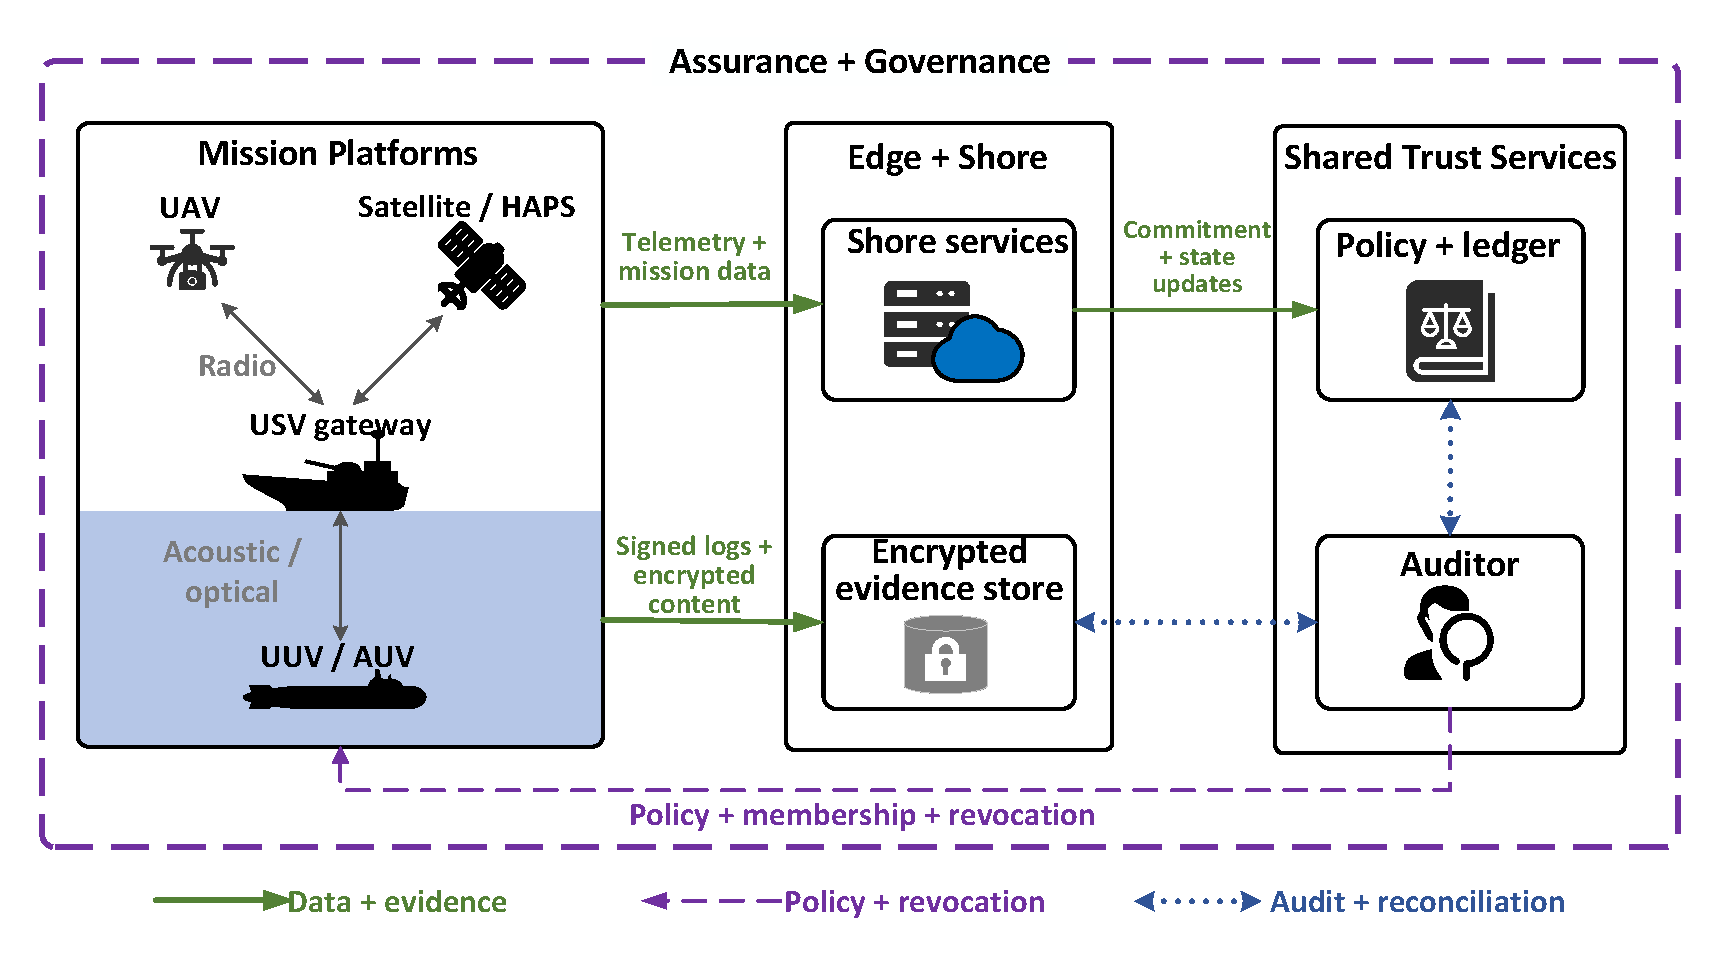
\includegraphics[width=\fulllength]{figures/figure-01-reference-architecture.pdf}

\end{adjustwidth}
\caption{\hl{Cross-domain} %MDPI: We moved Figure 1 into Sec. 3.2 to reduce blank, please confirm.
% Author response Q10 [RESOLVED]: The placement of Figure 1 in Section 3.2 is appropriate and has been retained.
 reference architecture. Shore organizations host peers and ordering nodes; the USV is a forwarding/cache dependency. Local sensing and safety continue within delegated authority during a gateway partition.\label{fig:architecture}}
\end{figure}





A \emph{\hl{trusted data environment}} is the socio-technical setting that produces, transforms, shares, and governs this evidence. It contains principals, devices, paths, artifacts, and accountability processes. Zero trust contributes resource-centered policy and enforcement~\citep{rose2020zero}; OAL records the additional observation, lineage, timing, and consequence claims relevant to mission reliance.

\subsection{Four Complementary Assurance Claims}

Observation validity concerns correspondence with the physical world. Commitment and provenance integrity concerns protected bytes and recorded origins or transformations. Ledger and governance consistency concerns authorized shared-state transitions. Mission-use suitability concerns the particular decision and consequence. Figure~\ref{fig:assurance-chain} shows the distinct questions and supporting evidence.


A forged observation signed with a stolen key can pass signature verification. RATS appraisals support scoped measured-state claims \citep{birkholz2023remote}, while physical diagnostics and corroboration support observation claims. The relying policy composes the applicable results, with explicit responses to failed or unknown requirements.

\begin{figure}[H]
\begin{adjustwidth}{-\extralength}{0cm}
\centering
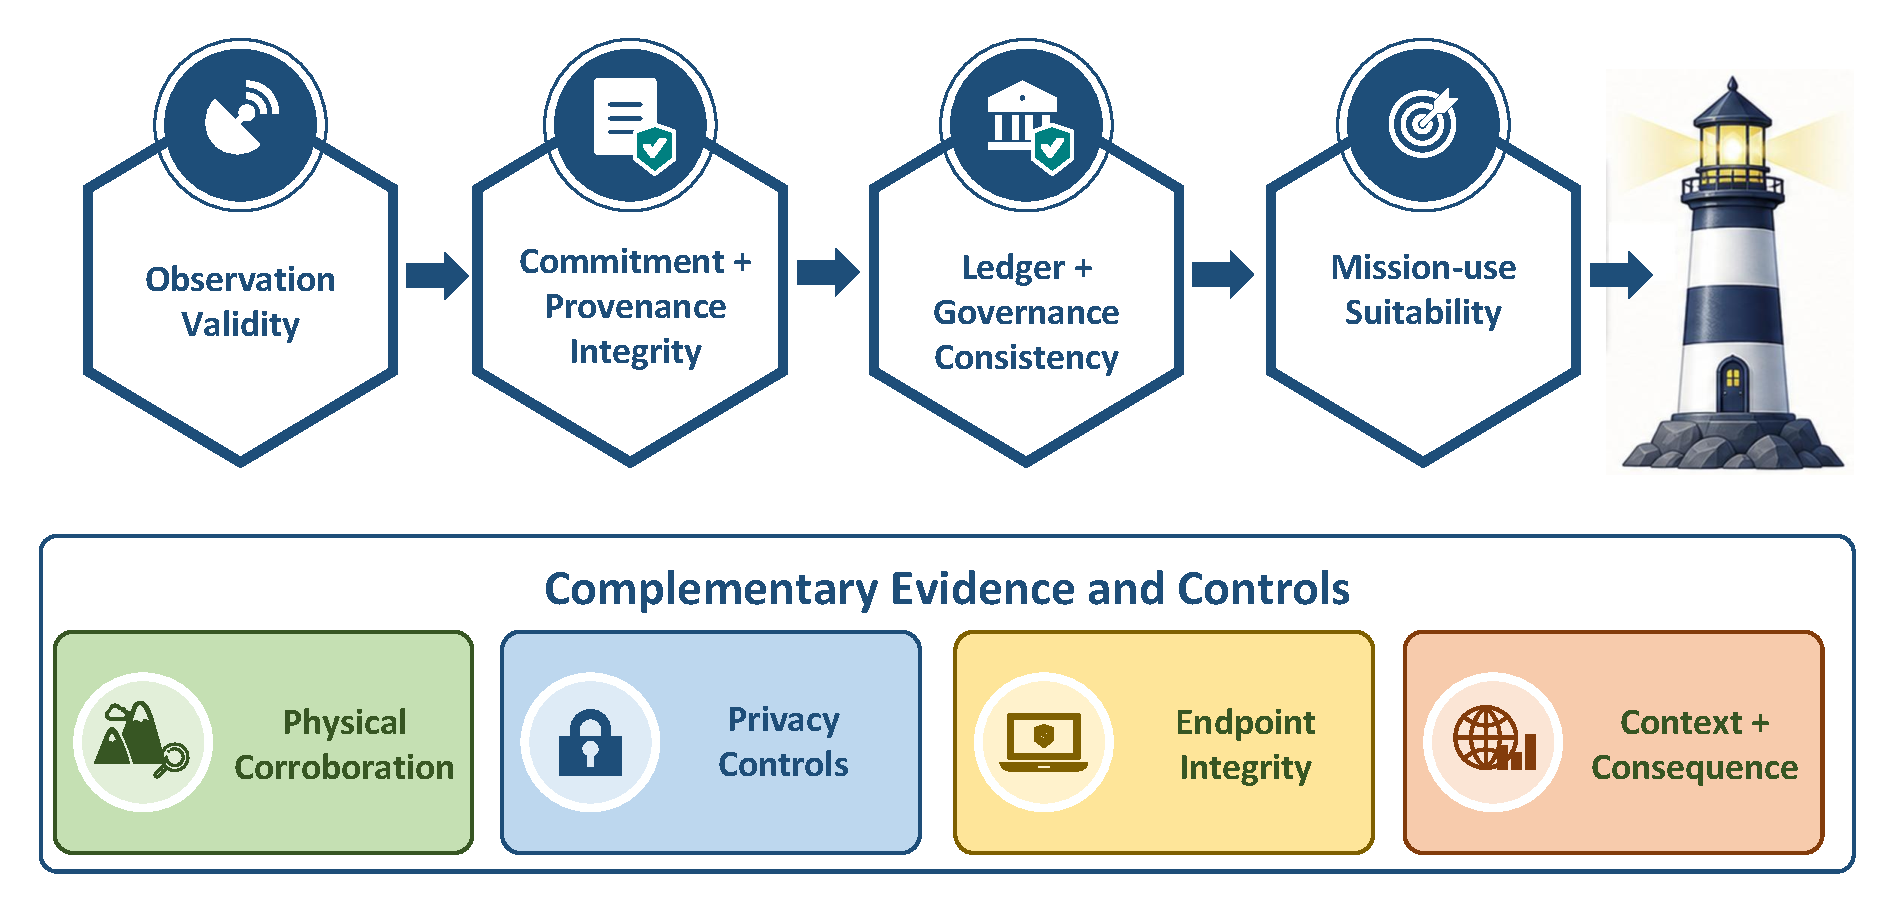
\includegraphics[width=\fulllength]{figures/figure-02-assurance-chain.pdf}

\end{adjustwidth}
\caption{Four assurance claims and their evidence. The relation is an argument structure; an implementation may evaluate the checks in a different order.\label{fig:assurance-chain}}
\end{figure}




\section{Complementary Research Landscapes}

Cooperative navigation and formation studies establish interactions among heterogeneous vehicles \citep{wu2020cooperative,ke2022cooperative,xue2021distributed,liu2023formation}. Their use of \emph{\hl{consensus}} concerns coordination of physical states. Ledger consensus concerns agreement on a replicated record under a fault model. OAL relates their outputs through identified observations, transformations, authorities, and intended uses.

\subsection{Security and Evidence Appraisal}

Security surveys organize spoofing, jamming, capture, malicious routing, malware, and false-data injection by target and attack mechanism \citep{yahuza2021internet,mekdad2023survey,jiang2019securing,adam2024state}. Underwater fading, noise, Doppler, and topology change can also cause loss or disagreement \citep{ali2020recent,jouhari2019underwater,mohsan2022towards}. A trust estimate therefore needs a named property and an uncertainty status: an anomaly may justify restricted use while its cause remains unresolved.

Decision-tree and hidden-Markov approaches illustrate underwater trust \linebreak  {inference~\citep{jiang2020dynamic,arifeen2020hidden}}. The former evaluates simulated network behavior with an initial attack-free training period; the latter includes a numerical illustration with ten generated observations. These studies support trust inference within their specified network and observation models. Reputation-based peer selection \citep{kamvar2003eigentrust} similarly supplies an appraisal mechanism whose meaning depends on the service and observed behavior. Survey taxonomies distinguish direct observations, recommendations, context, and attacks on reputation \citep{ahmed2019trust,aaqib2023iot,junior2021survey,liu2023survey}.

Observation appraisal supplies a complementary strand. Signal-feature classification, network-assisted detection, and recorded-data validation have been studied for GNSS spoofing \citep{shafique2021detecting,dang2022deep,semanjski2020use}. Multi-view opinion aggregation combines uncertain observations under declared assumptions \citep{liu2022trusted}. These methods address evidence about the physical world. Their outputs become inputs to a relying policy with a specified consequence and validity interval.

\subsection{Provenance, Attestation, and Access}

W3C PROV models entities, activities, and agents \citep{w3c2013provdm,w3c2013provo}. An OAL entity is an acting principal and usually maps to a PROV agent; an OAL data product maps to a PROV entity. Decision provenance extends the analysis along the data flows that lead to organizational or automated decisions \citep{singh2019decision}. It supports accountability when event capture and retained records cover the relevant transformations.

Attestation supplies measured endpoint-state evidence. Architectural proposals discuss attestation of ledger participants and autonomous IoT security \citep{hardjono2021towards,figueiredo2022arcadian}; implemented work evaluates attested channels and dual attestation of embedded devices and deployed ML artifacts \citep{ott2023universal,baciu2025secure}. RATS separates evidence, verifier appraisal, and the relying decision~ \citep{birkholz2023remote}. Zero trust and device baselines provide authorization and endpoint-capability requirements \citep{rose2020zero,syed2022zero,fagan2020iot}. These boundaries matter during disconnection, when cached results and delegated permissions age independently.

\subsection{Shared Records and Governance}

The coded UAV studies combine authenticated identities or data acquisition with ledger state \citep{han2022identity,tan2022blockchain,karmakar2024blockchain,islam2019bus}. Fabric provides an implemented execute--order--validate architecture~ \citep{androulaki2018hyperledger}; IoT platforms apply it to sensing-record integrity, off-chain provenance, and access policy \citep{hang2019design,honarpajooh2021iot,liu2020fabric}. Food, health, and digital-twin studies extend these patterns to forecasting, federated learning, and lifecycle coordination \citep{khan2020iot,rahman2020secure,suhail2022trustworthy}. Their recorded mechanisms and evaluation settings are summarized in Table~\ref{tab:reviews} and mapped in Section~\ref{sec:oal}.

\begin{table}[H]

\caption{The 39 coded studies and their principal evidence scope. Profiles apply to scoped claims and may overlap within a study.\label{tab:reviews}}
\begin{adjustwidth}{-\extralength}{0cm}
\footnotesize
\begin{tabularx}{\fulllength}{@{}P{25mm}P{46mm}P{24mm}Y@{}}
\toprule
\textbf{Identifiers} & \textbf{Mechanism Focus} & \textbf{Profiles} & \textbf{Evaluation Scope}\\
\midrule
S01--S04 & UAV identity/authentication/acquisition \citep{han2022identity,tan2022blockchain,karmakar2024blockchain,islam2019bus} & L1, L2, L3 & Security analysis, simulation and implemented components; BUS includes UAV and IoT hardware\\
S05--S07 & Underwater trust and P2P reputation \citep{jiang2020dynamic,arifeen2020hidden,kamvar2003eigentrust} & L1/L2 & Network or numerical evaluation and peer-selection simulation\\
S08--S10 & Fabric, sensing records, Hadoop provenance \citep{androulaki2018hyperledger,hang2019design,honarpajooh2021iot} & L3 & Server and embedded-device prototypes; record processing and retrieval\\
S11--S14 & Attestation and autonomous IoT security \citep{hardjono2021towards,ott2023universal,figueiredo2022arcadian,baciu2025secure} & L0 or L3 & Two architectural contributions; two implemented attestation studies\\
S15--S17 & Food/health provenance and access control \citep{khan2020iot,rahman2020secure,liu2020fabric} & L2 and/or L3 & Forecasting, FL applications and controlled access-policy requests\\
S18--S19 & Decision provenance and digital twins \citep{singh2019decision,suhail2022trustworthy} & L0 & Conceptual data-flow and lifecycle architectures\\
S20--S23 & GNSS and multi-view observation appraisal \citep{shafique2021detecting,dang2022deep,semanjski2020use,liu2022trusted} & L1/L2 & Signal/learning experiments, recorded data, and aggregation analysis\\
S24--S26 & Visual corroboration, UAV reports, fog offloading \citep{varshosaz2019spoofing,garcamagario2019security,alkhafajiy2020comitment} & L0/L2 & Recorded trajectories, agent simulation, and modeled partner/resource selection\\
S27--S29 & Maritime AIS provenance and message protection \citep{maritime2022monitoring,kessler2020protected,goudossis2022secais} & L3 & Receiver/ledger benchmark and two software protection demonstrations\\
S30--S31, S39 & UAV reputation, governance, and routing \citep{hierarchical2023trust,yang2023trusted,barka2022towards} & L0/L2/L3/L4 & Simulated trust updates; S31 includes a physical UAV-node experiment and a separate container testbed\\
S32--S34 & Underwater signcryption, routing, and FL \citep{zhang2026underwater,eetauv2025trust,tafl2026underwater} & L1/L2/L3 & Desktop cryptography, simulated routing and terrestrial-data proxy learning\\
S35--S38 & Generic consensus comparators \citep{hotstuff2019,narwhal2022,raft2014,pbft1999} & L1/L3 & Protocol reasoning and server/cloud prototypes; fault models and recovery paths differ\\
\bottomrule
\end{tabularx}
\end{adjustwidth}
\end{table}

The oracle problem remains relevant across these applications: a ledger preserves the accepted assertion and its provenance, while external validity depends on the data source and appraisal \citep{caldarelli2020oracle,albreiki2020oracles}. Transparency logs offer a natural alternative. Certificate Transparency specifies inclusion and consistency proofs, with external monitoring or witnessing needed to address inconsistent views \citep{rfc6962,rfc9162}. Sigstore combines signing with transparency for software artifacts \citep{sigstore2022}. A witnessed log can also carry jointly authorized state transitions. The distinction to evaluate is therefore the required validation and governance service, together with its implementation cost, rather than the presence of hash chaining alone.



\section{The OAL Framework and Literature Mapping}\label{sec:oal}

OAL classifies \emph{\hl{what is judged}}, \emph{\hl{which claim is sought}}, and \emph{\hl{when that claim is needed}}. A mechanism can support several cells; some combinations are inapplicable to a mission. Dependencies between claims are represented separately so that classification does not imply evidential independence.

\subsection{Objects, Assurance Layers, and Lifecycle}

An \emph{\hl{entity}} is an accountable principal: an organization, operator, service, or autonomous agent with delegated authority. A \emph{\hl{platform/device}} is the endpoint executing a function, including vehicles, gateways, sensors, and hosted compute instances. A vehicle can be considered an entity when exercising delegated authority and a platform when its firmware is measured. A \emph{\hl{link/path}} comprises physical media, intermediate nodes, security associations, and changing quality along an end-to-end route. A \emph{\hl{data product}} is an identified version of an observation, track, map, model, command, policy, or audit record. Corrections and transformations create new version identifiers. \hl{Table~{\ref{tab:objects}} summarizes the object-specific evidence and relying questions.}

\begin{table}[!htb]
\caption{\hl{OAL} %MDPI: Please cite this table in the text and ensure that the first citation of each table appears in numerical order.
% Author response Q11 [RESOLVED]: A highlighted citation of Table 3 has been added before the table in Section 5.1: "Table 3 summarizes the object-specific evidence and relying questions."
 objects and claim-specific evidence.\label{tab:objects}}
\begin{tabularx}{\textwidth}{@{}P{28mm}YY@{}}
\toprule
\textbf{Object} & \textbf{Evidence} & \textbf{Relying Question}\\
\midrule
Entity (E) & Credential, role, delegation, accountable actions & Who acts and with which authority?\\
Platform (P) & Boot/runtime measurements, configuration, self-test, energy & Which endpoint executes, and in what measured state?\\
Link/path (L) & Authentication, route, delay, loss, custody, and medium state & What protection and timeliness held along the path?\\
Data product (D) & Signature, content ID, times, lineage, uncertainty, residuals & Which version is this, and what supports its intended use?\\
\bottomrule
\end{tabularx}
\end{table}

The assurance axis uses O (observation validity), C (commitment and provenance integrity), G (ledger and governance consistency), and M (mission-use suitability). O uses physical bounds, calibration, diagnostics, and corroboration. C binds producer, version, and transformation assertions through signatures and provenance. G addresses jointly authorized membership, order, policy, and recovery state. M applies purpose, freshness, consequence, uncertainty, and authority requirements. When a shared-state service is not needed, ledger-specific claims are inapplicable; equivalent governance claims may be met by another service.


Policies, models, and reference values are versioned data products; their deployed instances reside on platforms, and their approval belongs to entities. This treatment makes the assurance infrastructure subject to the same analysis as mission observations. A cell specification identifies the object/version and required property, then gives the supporting evidence and validity interval. It also names the acceptance rule, responsible party, and response to missing evidence. \hl{Table~{\ref{tab:lifecycle}} summarizes the lifecycle stages and state transitions.}

\begin{table}[H]
\caption{\hl{Lifecycle} %MDPI: Please cite this table in the text and ensure that the first citation of each table appears in numerical order.
% Author response Q12 [RESOLVED]: A highlighted citation of Table 4 has been added before the table in Section 5.1: "Table 4 summarizes the lifecycle stages and state transitions."
 stages and relevant state transitions.\label{tab:lifecycle}}
\begin{tabularx}{\textwidth}{@{}P{35mm}YY@{}}
\toprule
\textbf{Stage} & \textbf{Required Assurance} & \textbf{Examples of Retained State}\\
\midrule
Admission (A) & Authorized principal and acceptable endpoint & Role, delegation, attestation reference\\
Sensing (S) & Credible time, place, and observation & Product ID, quality and acquisition commitment\\
Transmission (T) & Protected content and adequate path & Relay/custody event and batch root\\
Fusion/sharing (F) & Identified inputs, transformation and access & Lineage, model and policy version\\
Decision/action (D) & Fit for the specified consequence now & Decision rationale and responsible principal\\
Recovery/audit (R) & Scope of invalidation and restored authority & Revocation, dispute, reconciled history\\
\bottomrule
\end{tabularx}
\end{table}



\subsection{Observed Coverage in the Coded Sample}\label{sec:coverage}

Figure~\ref{fig:oal} maps 89 claims from 39 studies. Twenty-five of the 96 possible cells contain a coded claim. Data governance during processing/fusion (D/G/F) is the largest cell, with 16 studies. The 71 zero cells have no coded claim in this sample; their applicability depends on the mission. Cell counts also overlap: one study can protect a record, replicate it, and support its later audit.

The strata expose different emphases. Among 19 studies targeting UAV, maritime AIS, or underwater applications, entity governance at admission (E/G/A) is the largest cell, with six studies. Among 20 transferable studies, D/G/F leads with 11. Thus, the overall concentration partly reflects the inclusion of provenance and shared-state infrastructure. Each claim was checked against its supporting passage and evaluation setting.




\subsection{What the Comparison Changes in a Design Review}\label{sec:comparative}

The OAL axes separate the evidence supplied by a mechanism from the requirements of its next consumer. Table~\ref{tab:interfaces} compares mechanisms that share an application label or trust vocabulary but support different relying decisions. \hl{Table~{\ref{tab:sensitivity}} reports sensitivity to domain and coding choices.}

\begin{table}[H]
\caption{Claim boundaries exposed by the OAL comparison. The final column states the additional requirements for composing these mechanisms.\label{tab:interfaces}}
\begin{adjustwidth}{-\extralength}{0cm}
\small

\begin{tabularx}{\fulllength}{LLL}
\toprule
\textbf{Mechanism Comparison} & \textbf{Evidence Supplied} & \textbf{Consequence for Composition}\\
\midrule
AIS protection and receiver ledger (S27--S29) & Sender/message protection (E/C/T, D/C/T) and receiver-submitted history (D/C and D/G at F/R) have different trust boundaries & Preserve the original sender binding; require observation appraisal and freshness before using a position for action\\
Visual and multi-observer corroboration (S24--S25, S39) & Trajectory consistency or report agreement supports D/O at sensing/fusion under texture, geometry, and observer assumptions & Retain those assumptions with the result; authenticated agreement alone does not exclude correlated error\\
Attestation and partner selection (S12, S14, S26, S34) & Measured endpoint/model integrity differs from task-specific offloading or update suitability & Check both execution state and task evidence; neither credential nor trust score substitutes for the other's claim\\
UAV trust and routing (S30--S31, S39) & Changing behavior can trigger exclusion or path adaptation (E/M, L/M and E/G) & Reuse these continuity mechanisms, then specify authority and dependent-product handling across disconnection\\
Replicated-state protocols (S35--S38) & Similar D/G/F or D/G/R cells retain different fault models, synchrony and exercised recovery paths & Select assumptions before comparing latency; replicated-log recovery alone does not invalidate a derived mission product\\
\bottomrule
\end{tabularx}
\end{adjustwidth}
\end{table}

\begin{figure}[H]
\begin{adjustwidth}{-\extralength}{0cm}
\centering
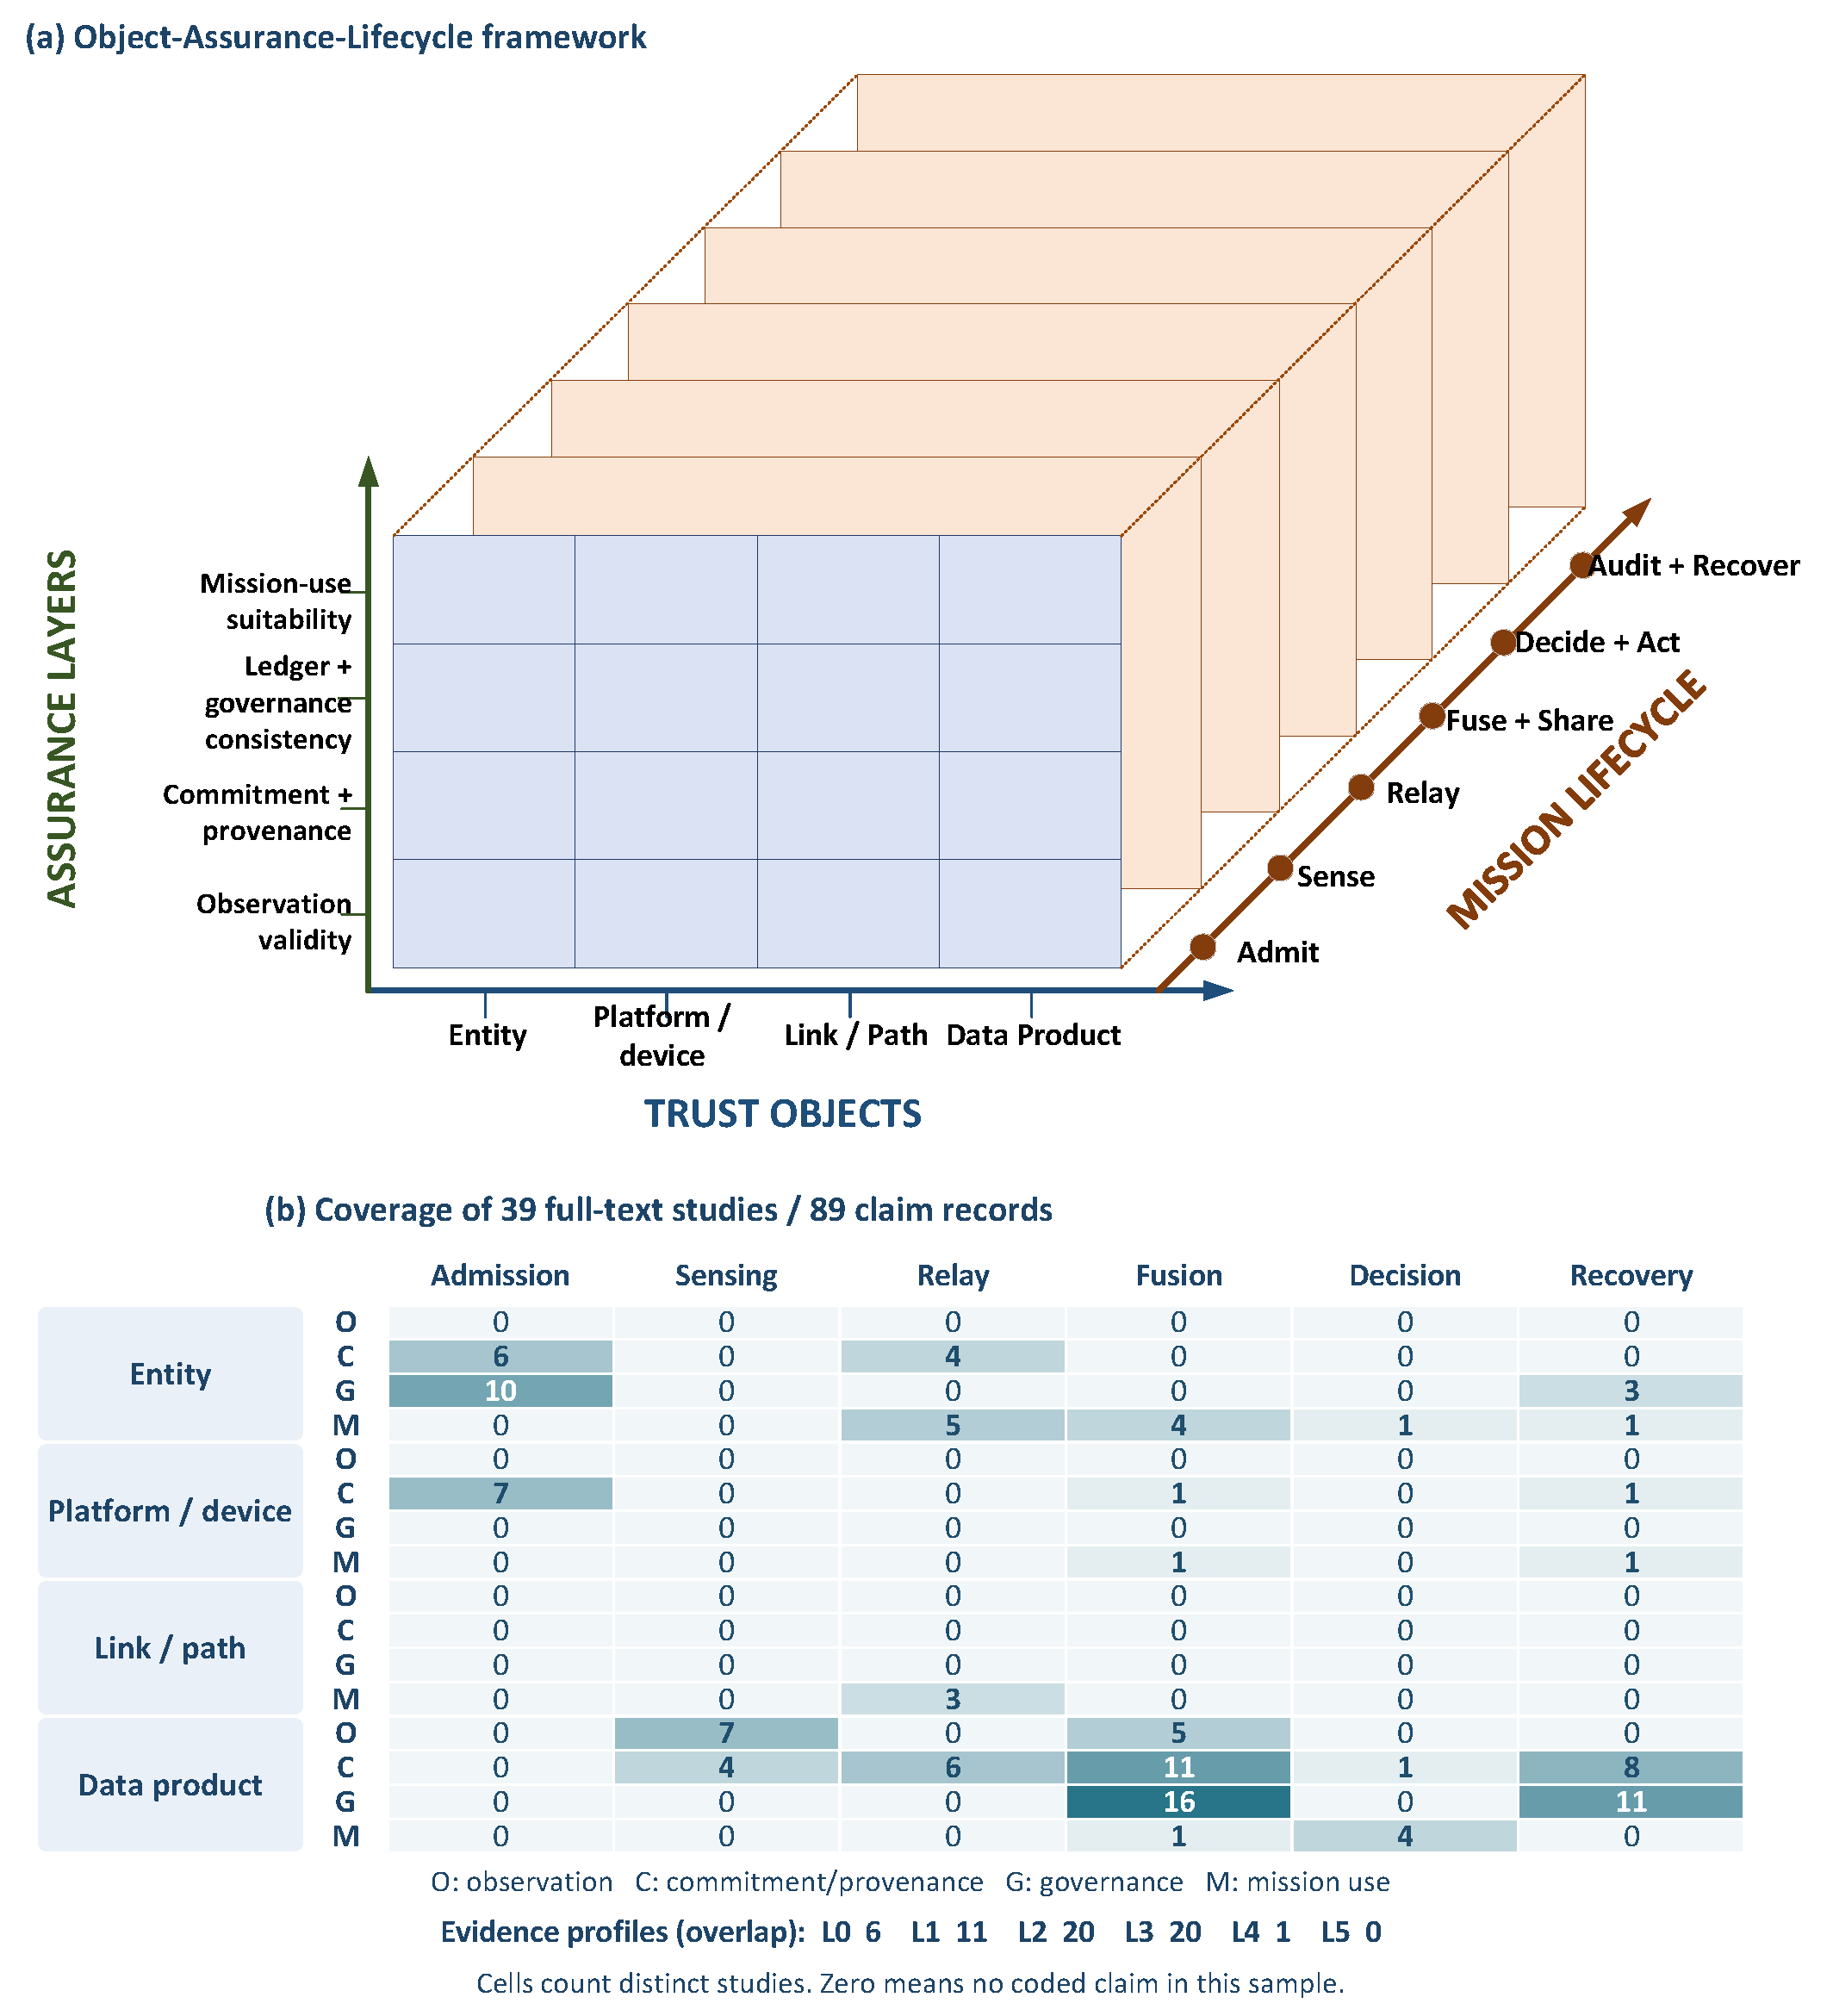
\includegraphics[width=\fulllength]{figures/figure-03-oal-framework.pdf}

\end{adjustwidth}
\caption{\hl{OAL} %MDPI: we moved Figure 3 into Sec. 5.3 to reduce blank, please confirm.
% Author response Q13 [RESOLVED]: The placement of Figure 3 in Section 5.3 is appropriate and has been retained.
 framework and mapping of 39 full-text mechanism studies. (\textbf{a}) The object, assurance, and lifecycle dimensions. (\textbf{b}) Distinct studies per exact cell, computed from 89 scoped claim records. Evidence-profile counts overlap. Zero denotes no coded claim, without establishing applicability or global research absence. Table~\ref{tab:sensitivity} separates domain and inclusion effects.\label{fig:oal}}
\end{figure}


\begin{table}[H]
\caption{\hl{Sensitivity} %MDPI: We moved the table below the first mention, please confirm.
% Author response Q14 [RESOLVED]: The production placement of Table 6 has been retained. A highlighted prose citation has been added in Section 5.3 before the Figure 3 caption and Table 6: "Table 6 reports sensitivity to domain and coding choices."
 of the coverage map. Occupied cells are descriptive counts, not a completeness score. D/G/F denotes data governance at fusion; E/G/A denotes entity governance at admission.\label{tab:sensitivity}}
\begin{tabularx}{\textwidth}{@{}YrrP{33mm}@{}}
\toprule
\textbf{Included Studies / Coding Variant} & \textbf{Studies} & \textbf{Cells} & \textbf{Largest Cell (Count)}\\
\midrule
All studies & 39 & 25 & D/G/F (16)\\
Direct-domain stratum & 19 & 18 & E/G/A (6)\\
Transferable stratum & 20 & 20 & D/G/F (11)\\
Without four generic consensus comparators & 35 & 25 & D/G/F (12)\\
Without conceptual-only studies & 35 & 22 & D/G/F (15)\\
Direct domain without proxy-data study & 18 & 17 & E/G/A (6)\\
Admission identities assigned only to entities & 39 & 25 & D/G/F (16)\\
Leave one study out (39 runs) & 38 & 23--25 & D/G/F (15--16)\\
\bottomrule
\end{tabularx}
\end{table}

The AIS comparison illustrates an assurance handover. The maritime monitoring prototype records observations submitted by authorized receivers \citep{maritime2022monitoring}; pAIS and SecAIS instead examine protection of AIS messages \citep{kessler2020protected,goudossis2022secais}. The pAIS demonstration uses weak demonstration parameters, while SecAIS implements selected modes with simulated AIS devices. Their L3 profiles identify software implementation, not equivalent security strength or on-air validation. A relying navigation service still needs evidence about the reported position. Visual-odometry cross-checking supplies one such mechanism, with recorded-data evaluation and limitations over low-texture water or at night \citep{varshosaz2019spoofing}. Multi-UAV corroboration supplies another under assumptions about observers and malicious participants \citep{garcamagario2019security,barka2022towards}. OAL exposes where a signed, consistently stored but erroneous position could otherwise pass an underspecified acceptance rule.

UAV trust and routing studies provide precedents for continuity. Hierarchical drone trust and blockchain-assisted routing update reputation and restrict cooperation as behavior changes \citep{hierarchical2023trust,yang2023trusted}. Yang et al. report a bounded experiment with eight physical UAV nodes, timed malicious forwarding, and a link interruption. This supports cooperation/path adaptation (L3/L4); their larger consensus benchmark uses a separate container environment. These mechanisms already connect observations of behavior to continued use. The additional coalition question concerns how a partitioned participant interprets changed authority and propagates invalidation to dependent products, as developed in Section~\ref{sec:trace}.

Task suitability is equally specific. COMITMENT combines partner history with workload/capacity criteria for fog offloading \citep{alkhafajiy2020comitment}. Underwater signcryption evaluates cryptographic operations on a desktop, while trust/energy routing uses simulation \citep{zhang2026underwater,eetauv2025trust}. TAFL-UWSN filters federated participants and updates, but its detailed evaluation uses terrestrial UNSW-NB15 data \citep{tafl2026underwater}. These results support distinct commitments or processing decisions; transferring them to an acoustic mission additionally requires channel, energy and data-distribution evidence.

Finally, a common cell does not imply interchangeable mechanisms. Raft and the Byzantine protocols differ in fault assumptions \citep{raft2014,pbft1999,hotstuff2019,narwhal2022}. The original PBFT prototype did not implement view changes or retransmissions, so its normal-operation claim receives L1/L3, and recovery receives L1. This claim-level distinction prevents a prototype label from spreading to an untested path. Across the sample, no extracted claim establishes an integrated air--surface--underwater mission with continuity of authority, observation appraisal, and dependent-product recovery all validated.

\subsection{Sensitivity to Selection and Coding}\label{sec:sensitivity}

Table~\ref{tab:sensitivity} summarizes how inclusion and coding choices change the coverage map. Removing the four generic consensus papers leaves all 25 occupied cells and the same leading cell, now with 12 studies. Removing the four conceptual-only studies reduces occupancy to 22. Thus, infrastructure comparators increase counts, while some coverage depends on conceptual mechanisms. The direct-domain pattern remains centered on admission governance when the terrestrial-data proxy study is removed.



Reassigning the S01--S03 platform-identity rows to entity identity changes individual cell counts without changing occupancy or the leading cell. Every leave-one-out map retains D/G/F as its largest cell, with 23--25 occupied cells overall. The L4 count depends on S31: coding its bounded physical-node experiment conservatively as a testbed removes L4 without changing the heatmap. The leading cell is stable to individual-study removal, while domain stratification and claim-level comparisons expose distinct composition requirements.


\section{Evidence Dependencies, Threat Propagation, and Dynamic Reasoning}

\subsection{A Typed Object-Dependency Graph}

Let $G_t=(V_t,E_t)$ be a time-indexed directed multigraph over OAL objects and their versions or state intervals. Relations name their semantics: an entity \emph{\hl{controls}} a platform; a platform \emph{\hl{hosts}} a model or \emph{\hl{produces}} an observation; a path \emph{\hl{transmits}} a product; an entity \emph{\hl{endorses}} or \emph{\hl{consumes}} a product; and a record \emph{\hl{commits to}} another product. A transformation links its inputs, output, executing platform, responsible entity, code/model version, and event interval. In PROV, this transformation can be serialized as an activity \citep{w3c2013provdm}. \hl{Figure~{\ref{fig:dependency}} shows these dependencies and their evidence states.}

\begin{figure}[!htb]
\begin{adjustwidth}{-\extralength}{0cm}
\centering
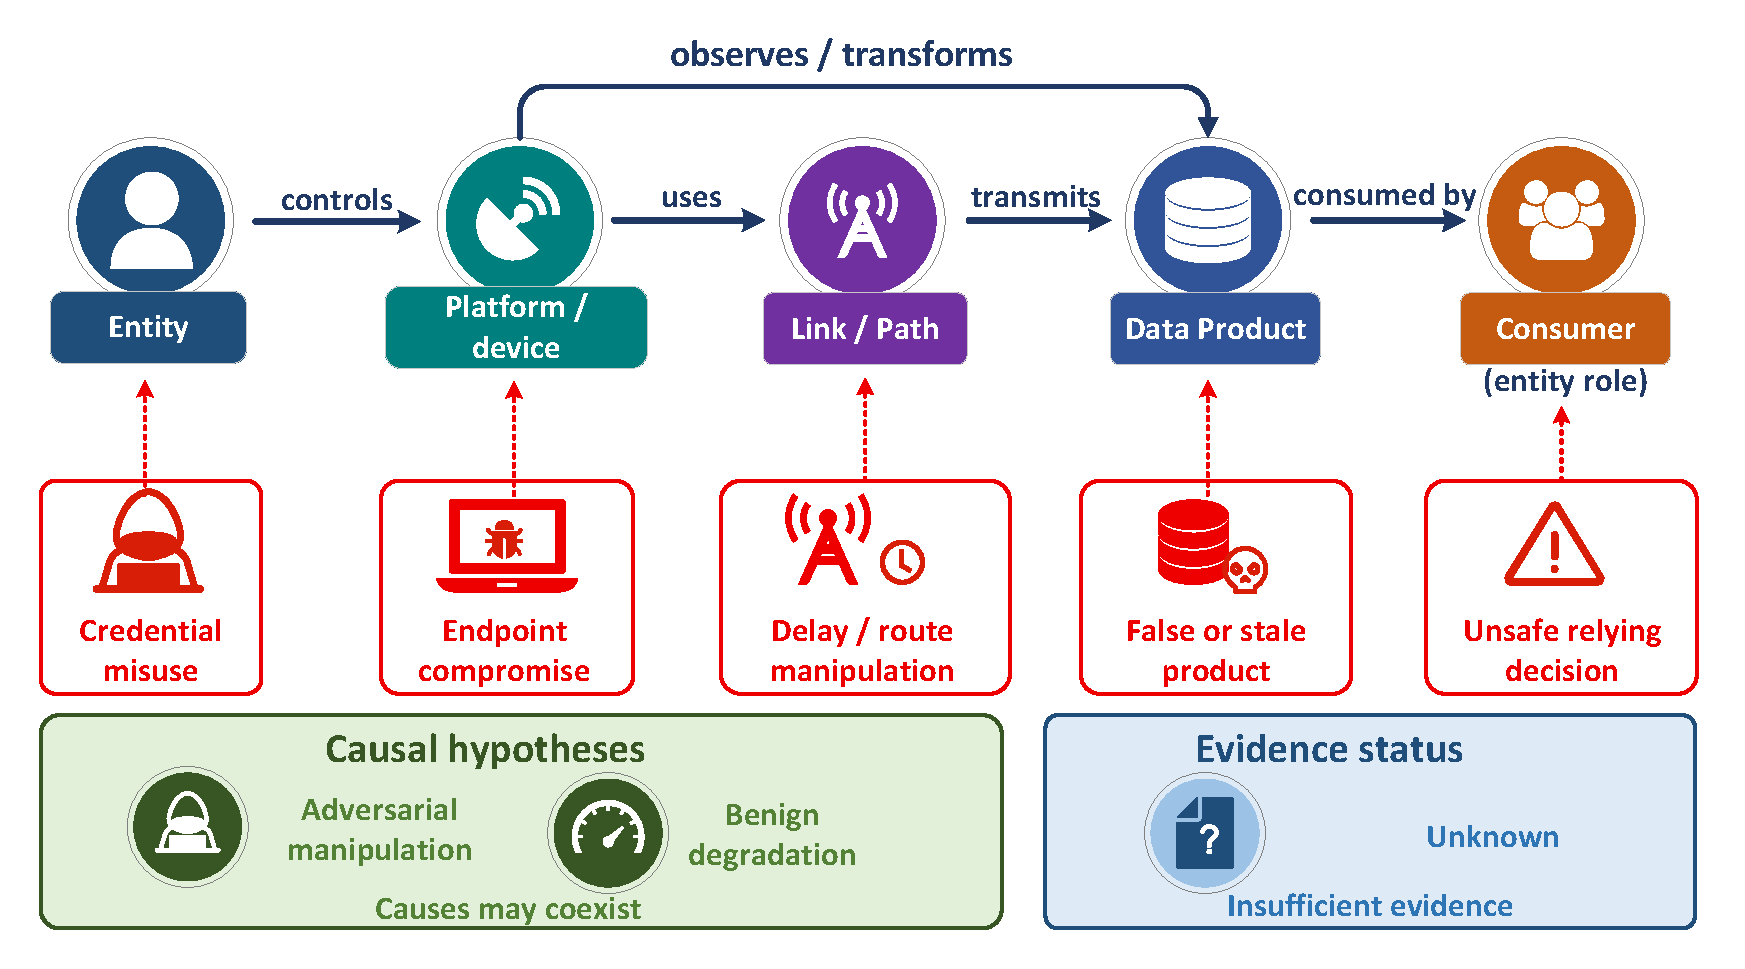
\includegraphics[width=\fulllength]{figures/figure-04-dependency-threat.pdf}

\end{adjustwidth}
\caption{\hl{Typed} %MDPI: Please cite this figure in the text and ensure that the first citation of each figure appears in numerical order.
% Author response Q15 [RESOLVED]: A highlighted citation of Figure 4 has been added before the figure in Section 6.1: "Figure 4 shows these dependencies and their evidence states." Figure citations first occur in numerical order.
 dependencies and evidence states. Operational relations identify claims affected by a changed assumption. Benign degradation and adversarial intervention are causal hypotheses; unknown is an epistemic outcome.\label{fig:dependency}}
\end{figure}

Traversal identifies claims for reassessment when a key, endpoint, model, or input becomes disputed. A graph edge alone does not quantify causal influence or justify a probability update. Corroboration must account for shared sources, clocks, transformations, and administrative roots. Two products derived from one observation do not supply two independent observations. Conversely, a shared relay need not invalidate end-to-end signatures from otherwise independent sources.

\subsection{Threats, Degradation, and Missing Evidence}

An analysis statement identifies the attacker or environmental cause and relevant capability, then traces the affected object and propagation relation to a mission consequence. It also records controls and residual uncertainty. For example, a compromised USV can withhold UUV batches, delaying the consumer's evidence and audit; independent contacts and protected local counters may expose gaps after reconnection. Acoustic fading can create the same delivery symptom with a different cause. The response can restrict freshness-sensitive use while attribution remains unknown. \hl{Table~{\ref{tab:threats}} summarizes selected cross-object failure paths.}

\begin{table}[H]
\caption{\hl{Cross-object} %MDPI: Please cite this table in the text and ensure that the first citation of each table appears in numerical order.
% Author response Q16 [RESOLVED]: A highlighted citation of Table 7 has been added before the table: "Table 7 summarizes selected cross-object failure paths."
 analysis of selected failure paths.\label{tab:threats}}
\begin{tabularx}{\textwidth}{LLL}
\toprule
\textbf{Initial Condition} & \textbf{Affected Dependency} & \textbf{Evidence and Response}\\
\midrule
Stolen credential & Entity authority to signed product & Effective-time revocation; review signed descendants\\
Compromised endpoint & Device state to observation or transformation & Attestation scope, diagnostics, corroboration; quarantine affected outputs\\
Fading or jamming & Path availability to evidence freshness & Channel/context evidence; restrict stale use and retain uncertain cause\\
Correlated sources & Shared input to fused conclusion & Lineage and common-cause model; reduce independent-evidence count\\
Unavailable governance quorum & Shared policy to fresh global authority & Retain prior checkpoint; enforce bounded local delegation\\
\bottomrule
\end{tabularx}
\end{table}

\subsection{The CTG Reasoning Loop}

CTG uses context, temporal state, and dependencies to guide appraisal and policy action through the eight-step loop in Figure~\ref{fig:ctg}. Evidence capture includes binding verification; propagation identifies affected descendants for reassessment under an explicit inference rule.



MAPE-K provides monitoring, analysis, planning, execution, and shared knowledge~\citep{kephart2003autonomic,ibm2005mapek}. CTG applies these functions to claim appraisal, separates event time from receipt time, and triggers reassessment through recorded dependencies. The JDL fusion model distinguishes object, situation, impact, and process refinement \citep{steinberg1999jdl}. For these estimates, CTG records the identity, provenance, governance, and temporal evidence needed for a relying decision.

Implementations can use Bayesian models, subjective logic, hidden-state inference, rules, or learned classifiers. Their outputs retain the named property, context, evidence lineage, uncertainty, and permitted use. Re-estimating trust after a change requires a specified update rule, rather than an arbitrary decrement along graph edges. A hard authorization condition can coexist with a graded quality estimate; the choice to make one condition non-compensable belongs to the mission policy.

\begin{figure}[H]
%\centering
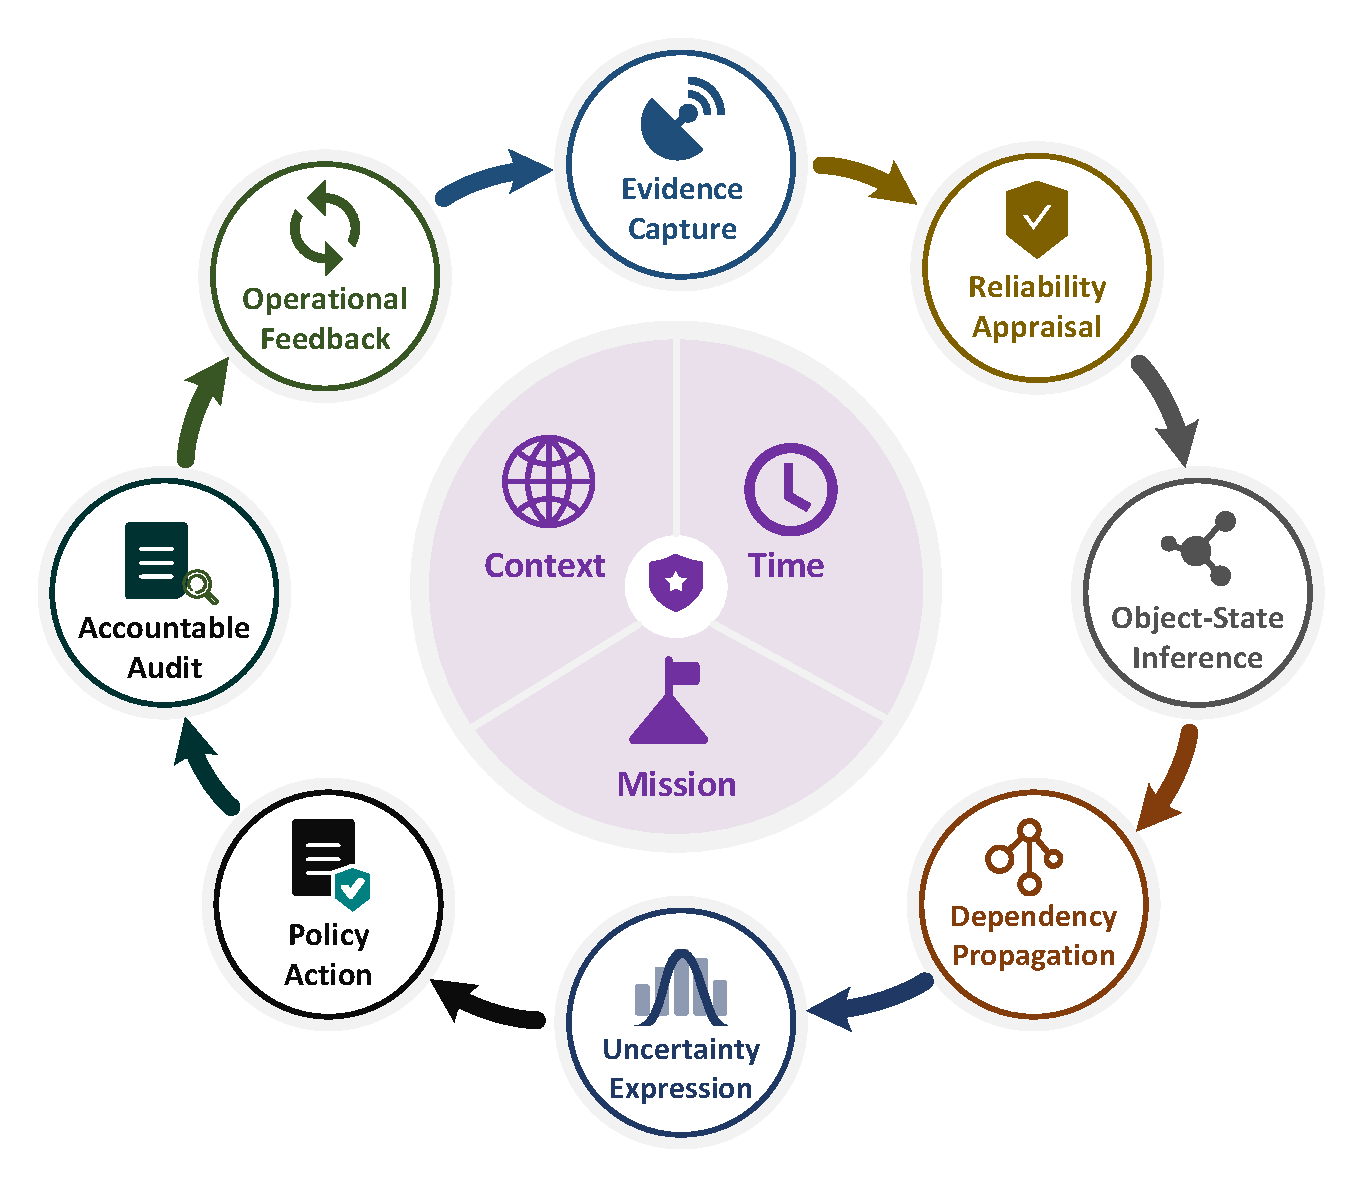
\includegraphics[width=0.90\textwidth]{figures/figure-05-ctg-reasoning-loop.pdf}
\caption{CTG appraisal and action loop, with policy, temporal state, and dependency knowledge shared across its steps.\label{fig:ctg}}
\end{figure}



\subsection{Partition, Revocation, and Reconciliation Trace}\label{sec:trace}

The coalition in Section~\ref{sec:coalition} has jointly approved policy version 1 and a low-consequence local delegation expiring at $t=480$ s. At $t=0$, the USV loses its shore connection; at $t=240$ s, shore organizations commit a revocation of a UUV signing key, effective immediately. The UUV receives the revocation at reconnection, $t=600$ s. Its protected clock reports event intervals, not exact event times. This scenario assumes a trustworthy pre-compromise time/counter record for the retained events; a stolen key alone cannot establish a credible historical timestamp.

Three signed records have intervals $[114,126]$, $[234,246]$, and $[294,306]$ s. On reconnection, a verifier checks their source signatures, batch inclusion, policy epoch, and the revocation history. A record whose interval ends before 240 s can be eligible for the historical audit. One beginning at or after 240 s is revoked at event time. An interval crossing 240~s is quarantined for review. Historical eligibility does not authorize a new physical action or refresh the observation.


The illustrative mean averages signature validity, observation quality, lineage, cached policy match, and temporal authority, using $[1,0.95,1,1,a]$ with $a=1,0.5,0$ and threshold 0.75. Its compensating aggregation accepts all three records. A scalar policy with an explicit authority veto produces exactly the typed rule's decisions. The decision difference follows from whether the policy enforces temporal authority as a veto. \hl{Table~{\ref{tab:trace}} reports the replay outcomes.}

\begin{table}[H]
\caption{\hl{Executable} %MDPI: Tables should appear in numerical order and below the first mention, so please revise the Table 8 citation.
% Author response Q17 [RESOLVED]: A highlighted first citation of Table 8 has been added in Section 6.4, before the table: "Table 8 reports the replay outcomes." The later citation in Section 9.2 remains a valid cross-reference.
 replay outcomes. Ledger and policy-validating witnessed-log paths use identical evidence and authorization rules. The scalar examples use the same input features.\label{tab:trace}}
\begin{tabularx}{\textwidth}{LLLL}
\toprule
\textbf{Event Interval (s)} & \textbf{OAL-Organized Rule / Validating Log} & \textbf{Mean Score} & \textbf{Scalar Decisions}\\
\midrule
114--126 & Eligible historical record & 0.99 & Mean accepts; veto-aware scalar agrees with rule\\
234--246 & Quarantine: revocation overlap & 0.89 & Mean accepts; veto-aware scalar quarantines\\
294--306 & Revoked at event time & 0.79 & Mean accepts; veto-aware scalar rejects\\
\bottomrule
\end{tabularx}
\end{table}



During disconnection, an action at 420 s can have restricted local authority under the cached envelope even though a later audit identifies a conflict with effective global revocation; at 540 s the envelope has expired and the local policy denies the action. Reconciliation retains both the locally available authority and the later global judgment. Rewriting the old decision as if the vehicle had received the revocation at 240 s would erase this distinction.

The synthetic replay verifies Ed25519 signatures and Merkle inclusion, rejects altered records/proofs, checks all six arrival orders with duplicate delivery, and enumerates all 16 coalition signer subsets. The ledger-policy and validating-log decision functions agree throughout. Section~\ref{sec:pattern} specifies how the same application rules map to Fabric and how the constrained vehicle receives an auditable result.



\section{Blockchain-Assisted Assurance: Selection and a Specified Pattern}

\subsection{The Decision to Use a Ledger}\label{sec:ledger-choice}

Ledger adoption begins with writers, state, and authority. W\"ust and Gervais organize the decision around the need to store shared state, the number and trust relationships of writers, and the availability of a trusted party \citep{wust2018need}. Locher et al. examine which functions of a trusted third party can be replaced by distributed agreement \citep{locher2018when}. For mission assurance, the relevant requirement is that no single organization may silently change accepted membership, policy, or revocation history, while authorized parties retain a mutually verifiable state.

In the coalition example, A alone must not replace a sensor-acceptance policy, C must not remove a previously acknowledged batch after a gateway incident, and D must not declare its own data accepted by the coalition. Four independent organizations can jointly validate those transitions. A permissioned ledger is one implementation of this requirement.

The strongest alternative is a transparency service whose checkpoints and state transitions are independently witnessed and checked under the same authorization rules. Such a service can satisfy the same safety requirements. A consistency-only witness detects or exposes inconsistent histories but does not by that act establish that a policy change was authorized. Adding joint policy validation closes that gap. The replay in Section~\ref{sec:trace} consequently finds equivalent decisions for the ledger and policy-validating log. Architecture selection then turns on implementation complexity, privacy, availability, recovery, and measured cost. \hl{Figure~{\ref{fig:blockchain-boundary}} summarizes this shared-state selection.}

Governance viability is also an adoption condition. Maersk and IBM discontinued TradeLens after it failed to achieve the required global industry collaboration and commercial viability, despite a technically viable platform \citep{maersk2022tradelens}. This maritime case motivates evaluating incentives, participation, exit, and operating responsibility.

\vspace{-3pt}
\begin{figure}[H]
\begin{adjustwidth}{-\extralength}{0cm}
%\centering
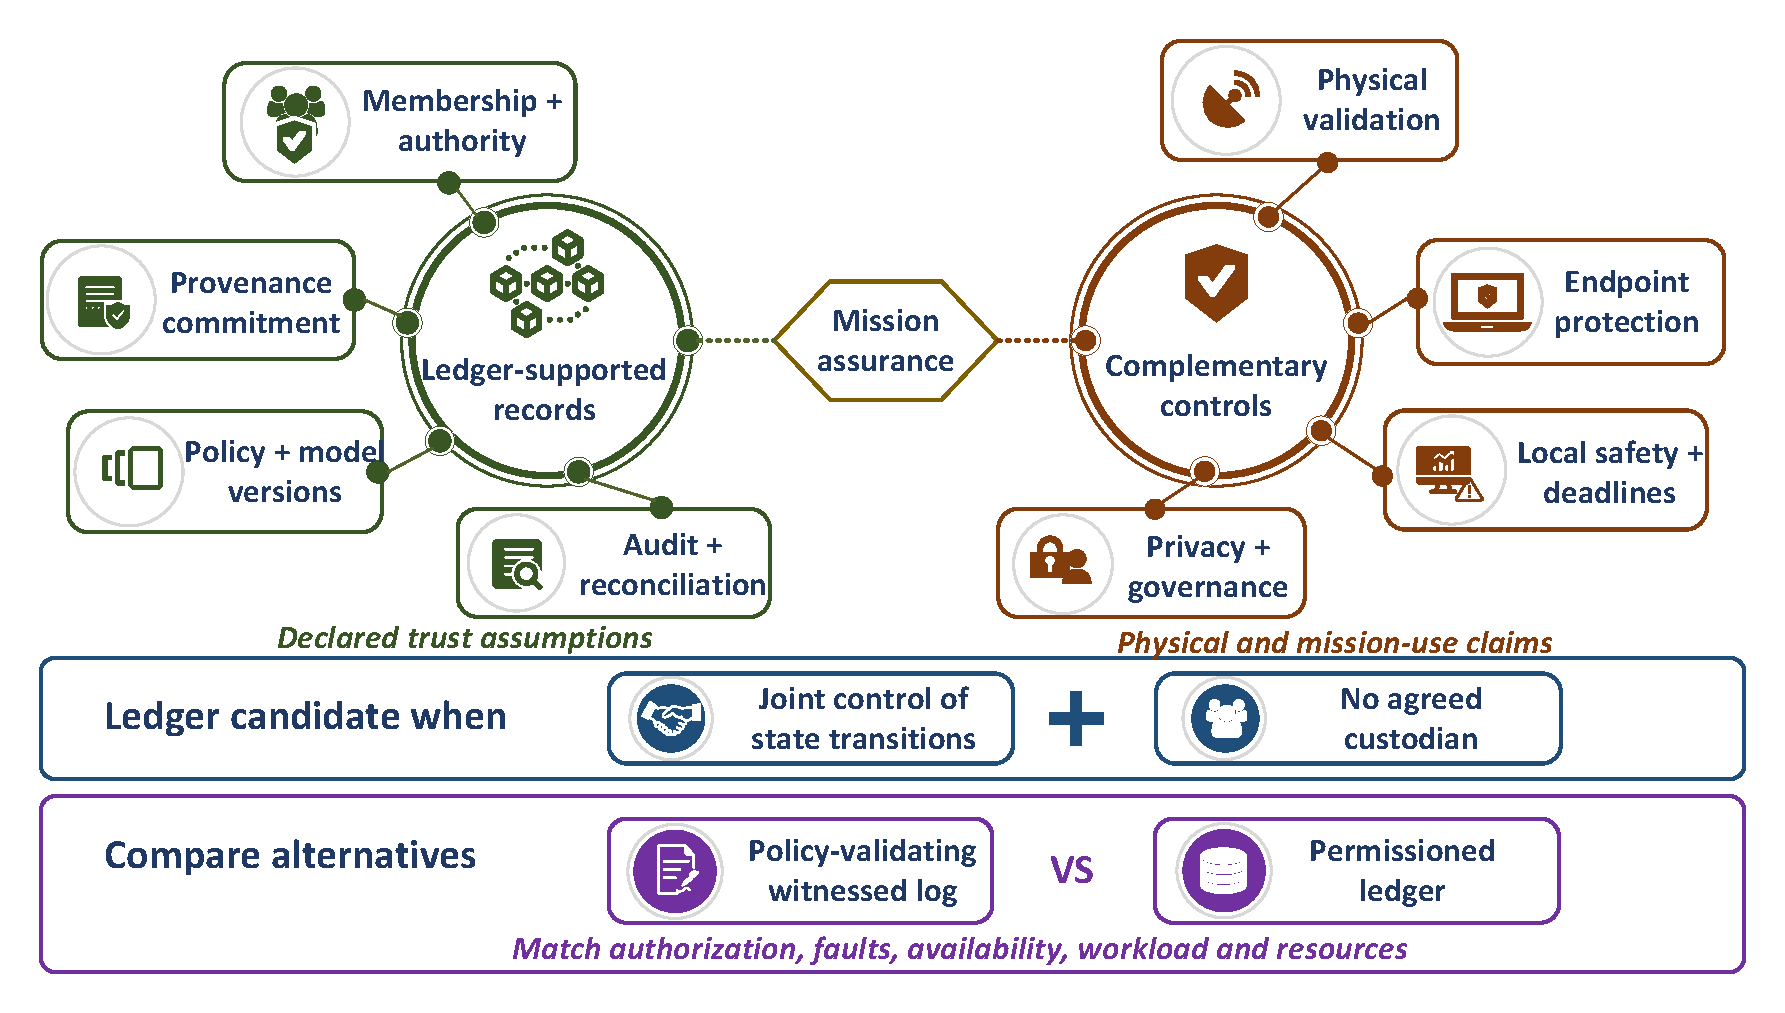
\includegraphics[width=\fulllength]{figures/figure-06-blockchain-boundary.pdf}

\end{adjustwidth}
\caption{\hl{Requirement}%MDPI: Please cite this figure in the text and ensure that the first citation of each figure appears in numerical order.
% Author response Q18 [RESOLVED]: A highlighted citation of Figure 6 has been added in Section 7.1 before the figure: "Figure 6 summarizes this shared-state selection."
-based shared-state selection. A policy-validating witnessed log and a permissioned ledger are compared under matched governance guarantees. Physical appraisal and local safety remain application responsibilities.\label{fig:blockchain-boundary}}
\end{figure}

\subsection{Mission Requirements and Consensus Candidates}\label{sec:consensus}

A requirement-based selection process, as advocated by \citet{svarcmajer2026consensus}, specifies the fault model before choosing a protocol. Here the coalition design assumes at most one Byzantine administrative domain among four independently controlled shore nodes. Safety must hold during a USV partition; new global decisions may stop when a responsive quorum is unavailable. The illustrative reconciliation deadline is 60 s after an event becomes available for shore processing. Membership is stable during a mission and changes through a jointly approved epoch transition. Shore nodes have adequate compute and power; UUVs do not participate in consensus. Consensus traffic uses shore/radio infrastructure, with only compact evidence commitments crossing the acoustic link.

Table~\ref{tab:consensus} compares representative families. Normal-path message complexity is a selection indicator, conditional on batching, signature aggregation, dissemination, and view changes. Fault tolerance and liveness assumptions remain decisive. In particular, a DAG organization does not remove the need to state which agreement protocol orders or certifies its data.


Raft and Byzantine protocols solve different fault problems \citep{raft2014,pbft1999,hotstuff2019}. CometBFT uses its own round-based consensus and gossip rules \citep{cometbft2026}; Narwhal is a dissemination/mempool component, while Tusk supplies an associated ordering protocol \citep{narwhal2022}. Authority-based UAV acquisition, as implemented in BUS, illustrates placement on capable validators \citep{islam2019bus}. Lightweight IoT proposals similarly motivate moving consensus away from constrained endpoints \citep{dorri2017towards}; the optimization must be assessed together with the resulting administrative dependencies.

\begin{table}[H]
\caption{Consensus candidates against the mission requirements. Message orders describe representative normal paths; recovery can cost more.\label{tab:consensus}}
\begin{adjustwidth}{-\extralength}{0cm}
\small
\begin{tabularx}{\fulllength}{LLLL}
\toprule
\textbf{Family} & \textbf{Fault Model and Partition Behavior} & \textbf{Latency, Traffic and Resource Implications} & \textbf{Scenario Fit}\\
\midrule
Raft & Crash faults; majority needed for progress & Leader replication, typically $O(n)$ exchanges per entry; low server cost; managed membership & Single accountable operator with crash-only replicas; insufficient for Byzantine coalition administrators\\
Classical BFT / SmartBFT & Byzantine faults; typically $n\geq3f+1$ and $2f+1$ responsive votes & Multi-phase communication, commonly $O(n^2)$; timeout/view-change cost; capable stable nodes & Small independent shore coalition; selected Fabric ordering candidate\\
HotStuff & Byzantine faults; quorum and partial-synchrony liveness & Linear normal-path communication with quorum certificates and pipelining; cryptographic aggregation and leader availability matter & Larger capable coalition with measured load benefit\\
CometBFT & Byzantine faults; more than two-thirds voting power; round/locking rules & Tendermint-style propose/vote and gossip; timeouts under delay; implementation-dependent dissemination cost & Application-specific replicated state machine; not classified as HotStuff merely because both use BFT\\
Authority-based & Named validators; resilience depends on the actual protocol & Low mining cost; schedule/finality and quorum assumptions must be identified & Controlled consortium only after the concrete authority protocol meets the fault requirement\\
DAG-based (Narwhal/Tusk) & Reliable data dissemination plus an explicit BFT ordering protocol & Parallel dissemination and storage; asynchronous progress assumptions and communication cost remain & High-throughput shore service with resource evidence; no acoustic-partition shortcut\\
IoT-oriented designs & Often cluster heads, trusted managers, or restricted validator sets & Reduce endpoint work by moving it to capable nodes; altered trust and availability assumptions & Gateway-mediated collection; selected only if its delegated trust matches the mission\\
\bottomrule
\end{tabularx}
\end{adjustwidth}
\end{table}



Fault assumptions are stated separately for infrastructure and applications. A Byzantine ordering service concerns agreement despite arbitrary behavior of replicas; it does not prevent an authorized producer from supplying a false observation. Endorsement constrains who approves a proposed state update, while the chaincode defines the deterministic rule being approved. A contract can consistently implement an unsuitable rule, so policy approval also requires evidence about its mission consequence. The application must specify whether emergency authority can bypass ordinary endorsement and how that exception is recorded and reviewed. Without an explicit exception, loss of a mandatory signer is an intentional loss of fresh global authorization.

Partition tolerance likewise has two meanings that must be separated. Safety preserves a consistent accepted history when messages are delayed or unavailable. Availability concerns whether a particular request can obtain the needed ordering and application approvals before its deadline. A shore quorum may remain healthy while the USV is disconnected, allowing shore revocations to progress while a UUV continues under cached authority. If the shore quorum itself is divided, new global updates may stop even after the gateway returns. Evaluations should vary these two partition locations independently. Classical consistency/availability results motivate this distinction under network partition~\citep{gilbert2002brewer}; they do not specify the vehicle's local safety policy.

Three scenario decisions follow. A single-agency inspection mission can use an authenticated database or witnessed log, adding Raft replication for crash availability. The four-organization response mission requires Byzantine ordering plus joint application authorization, or an equivalent validating log; current Fabric SmartBFT is a concrete candidate~\citep{fabric2026bft}. A disconnected UUV group uses signed local records, store-and-forward transport, and bounded delegation, with no requirement for acoustic consensus. Increasing validator count only helps when it increases independent fault domains while preserving a reachable quorum. Actual latency and energy must be measured for the selected deployment.

\subsection{A Coalition Provenance-And-Revocation Pattern}\label{sec:pattern}

The specified pattern combines evidence commitments and post-partition reconciliation; Table~\ref{tab:blockchain-patterns} relates these to membership, version coordination, and audit.

\begin{table}[!htb]
\caption{Ledger roles and their corresponding application requirements.\label{tab:blockchain-patterns}}
\begin{tabularx}{\textwidth}{LLL}
\toprule
\textbf{Role} & \textbf{Shared State} & \textbf{Required Complementary Evidence}\\
\midrule
Membership & Role, delegation, key epoch & Identity proof and protected key custody\\
Commitments & Batch root, sequence, retained-object reference & Signed source records and retrievable payload\\
Version coordination & Policy/model hash and approval epoch & Model validation and deployment evidence\\
Audit & Decision, evidence links, and effective-time history & Complete capture and independent review\\
Reconciliation & Received batch, gaps, conflicts, judgments & Protected clock/counter and offline-authority history\\
\bottomrule
\end{tabularx}
\end{table}

\textbf{\hl{Placement and endorsement.} %MDPI: Please confirm if the bold formatting is necessary; if not, please remove it. The following highlights are the same.
% Author response Q19 [RESOLVED]: Please retain the highlighted bold formatting. The phrases in Section 7.3 function as paragraph headings; P1--P6 in Section 9.2 identify the six testable propositions. Their formatting is consistent within each group.
} Each organization A--D hosts an endorsing peer and a separate ordering node on capable shore infrastructure. The illustrative BFT service has four orderers, tolerating one Byzantine node under its protocol assumptions. Administrative separation supplies the independent fault domains. The application endorsement rule is \texttt{\hl{AND(A, B, OR(C, D))}%MDPI: Please confirm whether the special font should be retained, same as below.
% Author response Q20 [RESOLVED]: Please retain the monospace font for AND(A, B, OR(C, D)) and the function identifiers CommitBatch, JudgeRecord, UpdatePolicy, and RevokeKey. These are policy expressions and interface identifiers, so the font distinguishes them from ordinary prose.
}; channel configuration and chaincode-definition approval require the same coalition authority. A and B are mandatory, so application progress can stop even while three orderers remain responsive. The USV forwards and caches signed evidence, with no consensus vote. A partitioned gateway buffers batches and retries idempotently after reconnection. UUV safety control uses its local envelope throughout.

\textbf{\hl{State and encoding.}} The state keys are mission/policy/epoch, producer/key/history, delegation/identifier, batch/producer/sequence, and judgment/record/policy. The fixed-width source body contains one byte each for version and type, two 16-byte mission/producer identifiers, four-byte sequence and authority-epoch fields, two eight-byte event-time bounds, and three 32-byte hashes for policy, payload, and parent/root. These fields total 154 bytes. Integers use network byte order; time is signed seconds in the declared mission epoch. A 64-byte Ed25519 signature gives a 218-byte record. Domain-separated signing and hashing bind record type and version. A batch uses the same body layout with a Merkle root and previous-batch root, plus a two-byte record count: 156 bytes before signature and 220 bytes signed. Ten signed records are retained off chain. The gateway's canonical JSON application payload is 525 bytes.

\textbf{\hl{Deterministic chaincode operations.}} \texttt{\hl{CommitBatch}} reads the mission epoch, gateway role, and last batch sequence; verifies the compact gateway signature and policy binding; rejects an inconsistent sequence or duplicate identifier with different content; and records the root. An identical retry returns the existing result. This commits an auditable batch, not a claim that every leaf is fit for use. \texttt{\hl{JudgeRecord}} verifies a supplied source signature and inclusion proof, reads the producer's historical key status and delegation, and writes a separate eligible/revoked/quarantined judgment using the interval rule in Section~\ref{sec:trace}. \texttt{\hl{UpdatePolicy}} and \texttt{\hl{RevokeKey}} require the coalition endorsement rule and monotone epochs; revocation records preserve their effective time. All state that is read for a decision enters the Fabric read set, allowing validation to reject stale concurrent updates. Chaincode obtains no external clock or oracle value during execution; authorized submitted evidence supplies those inputs.

\textbf{\hl{Commit status and constrained verification.}} Fabric ordering precedes peer validation, so block inclusion is not proof of a valid world-state update \citep{androulaki2018hyperledger,hyperledger2026fabric}. After observing a valid commit, three distinct organizations satisfying A+B+(C or D) sign an application receipt containing the mission, policy/authority epoch, batch root, sequence, event span, and count. Receipt-signing code must check the commit validation status and the expected application state. A UUV checks authorized signer identities against its pinned epoch, signatures, monotone checkpoint sequence, source-record signature, and the Merkle branch. For ten leaves padded to 16, the branch has four 32-byte hashes. These checks establish a jointly attested application checkpoint and inclusion under pinned keys; they do not constitute native verification of all Fabric consensus and peer-validation execution. A new epoch requires an authenticated transition from the pinned epoch. The receipt is an additional application trust boundary that must be implemented and tested.

\subsection{Communication Budget and Partition Sensitivity}\label{sec:budget}

The receipt and retrieval paths serve different evidence needs. A vehicle receiving a checkpoint can verify that independent organizations acknowledged the committed root under a pinned authority epoch. To appraise an observation, it still obtains the relevant leaf, its inclusion path, and any required source or transformation evidence. A commitment-only contact therefore supports a narrower claim than complete evidence delivery. Retrieval policy can prioritize recent high-consequence products and defer bulk imagery until a higher-bandwidth contact, while recording which required inputs remain unavailable. A failed retrieval is represented as missing evidence rather than a successful integrity check.

Clock and key transitions also affect the usable lifetime of a proof. A cached checkpoint remains evidence about a historical commitment after a new policy is issued, but its authority to support a new decision depends on the relying policy and authenticated transition history. A vehicle with an uncertain clock cannot establish that an expiry condition still holds by inspecting a ledger root. It needs a bounded time interval or a more restrictive fallback. Similarly, a fresh receipt cannot make an untrustworthy acquisition timestamp credible. These requirements bind the application-level proof to the same temporal assumptions used in the replay and define what a constrained verifier must do when those assumptions fail.

Ed25519 signatures contain 64 bytes \citep{rfc8032}; ML-DSA-44 signatures contain \linebreak  2420~bytes~\citep{fips204}. The budget compares these two compact application signature profiles. Fabric enrollment certificates, endorsements, proposal responses, read/write sets, and envelopes add deployment-dependent bytes. Only the gateway transports those full transactions on the shore network. Full transaction sizes and resource costs depend on the configured Fabric implementation; the 525-byte JSON value covers the gateway's application payload.

For a message of $B$ bytes and net payload rate $R$ bit/s, the serialization lower bound \hl{is} %MDPI: please confirm whether ``B/R'' is unit, if so, please remove italic for units.
% Author response Q21 [RESOLVED]: B and R are variables, not unit symbols: B is the message size in bytes and R is the net payload rate in bit/s. The lower bound is 8B/R seconds. The variables remain italic, while the units bytes, bit/s, and seconds remain upright.
 $8B/R$. Table~\ref{tab:budget} uses 100, 1000, and 5000 bit/s as scenario inputs. It excludes propagation, contact waiting, modem framing, BPSec overhead, loss, retries, and certificate/epoch updates. Those factors increase end-to-end delay and must be added for a specified modem and transport configuration.

\begin{table}[!htb]
\caption{Application-message serialization lower bounds. All sizes are computed from the encoding in Section~\ref{sec:pattern}; ML-DSA values substitute the standardized signature length.\label{tab:budget}}
\begin{tabularx}{\textwidth}{@{}Yrrrr@{}}
\toprule
\textbf{Message} & \textbf{Bytes} & \textbf{100 bit/s} & \textbf{1 kbit/s} & \textbf{5 kbit/s}\\
\midrule
Ed25519 source record & 218 & 17.44 s & 1.744 s & 0.349 s\\
Ed25519 batch commitment (10 records) & 220 & 17.60 s & 1.760 s & 0.352 s\\
Ten complete Ed25519 records & 2180 & 174.40 s & 17.440 s & 3.488 s\\
ML-DSA-44 batch commitment & 2576 & 206.08 s & 20.608 s & 4.122 s\\
Ed25519 record + branch + joint receipt & 697 & 55.76 s & 5.576 s & 1.115 s\\
\bottomrule
\end{tabularx}
\end{table}

The 697-byte downlink comprises a 218-byte source record, 128-byte branch, two-byte leaf index, 156-byte checkpoint, one-byte signer bitmap, and three 64-byte signatures. At one ten-record batch per minute, the 220-byte commitment needs about 29.3 net bit/s on average, whereas sending all ten signed records needs about 290.7 bit/s. Commitment-only delivery therefore fits some contacts that cannot carry full evidence, at the cost of later retrieval and incomplete immediate appraisal. Sending one ten-record ML-DSA-44 batch commitment at the same cadence requires about 343.5 bit/s. Public keys are assumed provisioned; key distribution and post-quantum verification time remain separate costs.

The partition sensitivity calculation covers 63 configurations: validator counts of 4, 7 and 10; responsive counts of quorum minus one, quorum, and all validators; and partition durations of 0, 10, 30, 58, 59, 60, and 120 s. With assumed post-contact delays of 2 s for a ledger path and 1 s for a validating-log path, a 60 s deadline permits partitions of at most 58 and 59 s, respectively, when a quorum is reachable. Below quorum, neither completes a fresh joint decision. Application endorsement availability must be checked in addition to ordering quorum.


\section{Evaluation Practices and Evidence Maturity}

\subsection{A Claim-Specific Evidence Profile}

L0--L5 record how a claim is supported: concept, analysis, simulation/data, prototype, field trial, and sustained operation. Figure~\ref{fig:maturity} relates each evidence form to its inputs, reasoning or evaluation, and outputs. Formal soundness, experimental control, environmental representativeness, and operational duration remain separate assessment dimensions.

\begin{figure}[!htb]
\begin{adjustwidth}{-\extralength}{0cm}
\centering
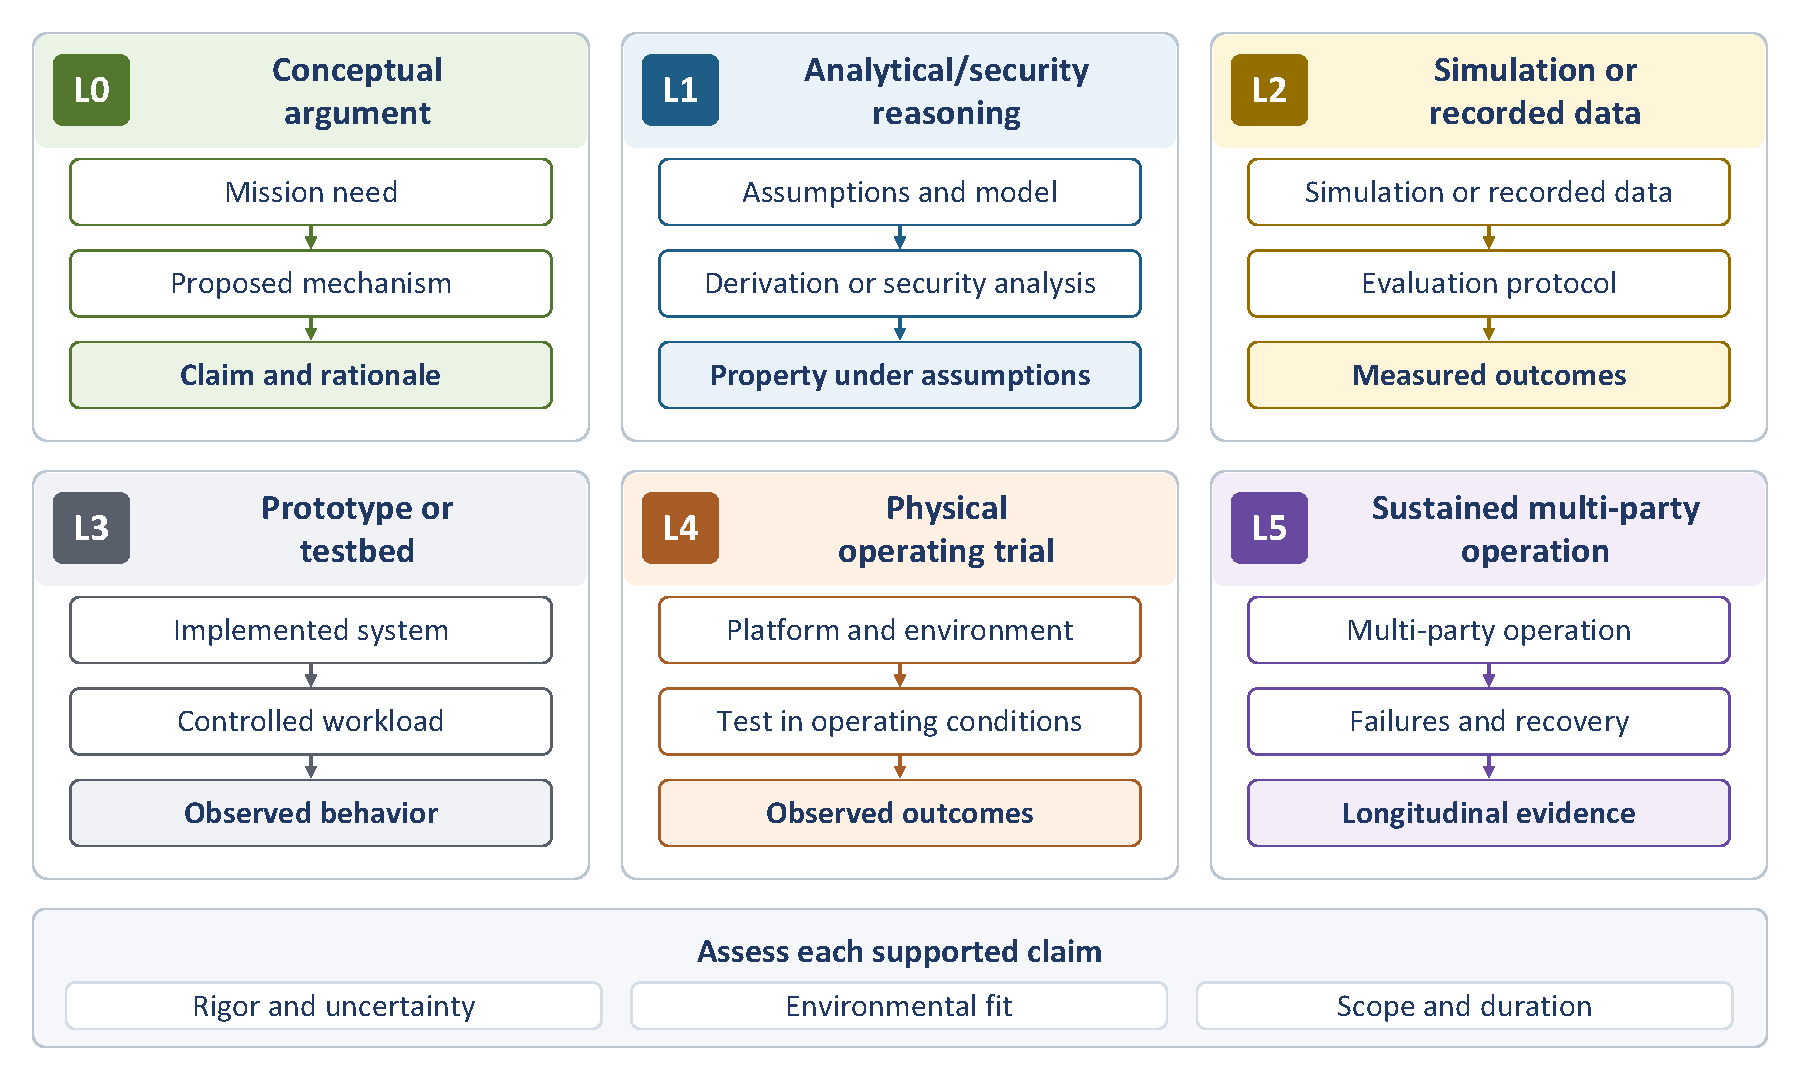
\includegraphics[width=\fulllength]{figures/figure-07-evidence-maturity.pdf}

\end{adjustwidth}
\caption{\hl{Complementary} %MDPI: we moved it here to reduce blank, please confirm.
% Author response Q22 [RESOLVED]: The production placement of Figure 7 in Section 8 has been retained.
 evidence forms and their claim-specific support. Each panel relates inputs, reasoning or evaluation, and outputs; rigor, environmental fit, and scope are assessed separately.\label{fig:maturity}}
\end{figure}

Within the 39-study sample, six profiles include L0, eleven L1, twenty L2, twenty L3, and one L4; none includes L5. Profiles overlap; four studies are conceptual-only. The L4 assignment concerns S31's bounded physical UAV-node cooperation/routing experiment; its container consensus benchmark remains L3. Treating that experiment as L3 only is evaluated as a sensitivity variant in Section~\ref{sec:sensitivity}. BUS supplies hardware-prototype evidence, while recorded GNSS trajectories support L2. These settings answer different questions about implementation, physical operation, and transfer.

As the comparisons in Section~\ref{sec:comparative} show, evidence form, parameter strength, exercised mechanism, and environmental relevance jointly determine the supported claim.

\subsection{Datasets, Simulators, and Testbeds}

Public resources support complementary evaluation tasks. CICIoT2023, TON\_IoT, and Edge-IIoTset supply attack and telemetry data for classification and robustness\linebreak   tests~\citep{neto2023ciciot2023,alsaedi2020ton,ferrag2022edge}. SeaDronesSee supplies maritime visual data \citep{varga2022seadronessee}. AirSim, UUV Simulator, and Aqua-Sim NG address vehicle/sensor simulation, underwater dynamics, and underwater communication, respectively \citep{shah2018airsim,manhaes2016uuv,martin2017aqua}. Their use in one experiment requires compatible clocks, geometry, mobility, and event interfaces, together with a separately validated mission-loss model. \hl{Table~{\ref{tab:evaluation}} summarizes the resources and transfer checks.}

\begin{table}[H]
\caption{\hl{Evaluation} %MDPI: Please cite this table in the text and ensure that the first citation of each table appears in numerical order.
% Author response Q23 [RESOLVED]: A highlighted citation of Table 12 has been added before the table: "Table 12 summarizes the resources and transfer checks." All table first citations have been checked in numerical order.
 resources and required transfer checks.\label{tab:evaluation}}
\begin{tabularx}{\textwidth}{LLL}
\toprule
\textbf{Resource} & \textbf{Useful Evidence} & \textbf{Required Complement}\\
\midrule
IoT attack/telemetry datasets & Detection, calibration, missingness and false isolation & Maritime topology, benign degradation and mission consequences\\
SeaDronesSee / GNSS recordings & Visual detection or signal appraisal & Independent ground truth for the stated physical claim\\
AirSim / UUV Simulator & Dynamics, sensors, disturbance and control & Field validity of the configured models\\
Aqua-Sim NG & Path delay, loss, energy and contact behavior & Physical observation and governance modules\\
Ledger and witnessed-log testbeds & Validation, bytes, latency, recovery and membership changes & Matched guarantees, evidence workload and fault domains\\
Multi-organization field exercise & Integrated decisions, recovery and audit & Repeated scenarios and explicit operational duration\\
\bottomrule
\end{tabularx}
\end{table}

\subsection{Metrics, Baselines, and Reproducibility}

An evaluation should measure inference error and uncertainty, mission consequences, network/resource cost, shared-state behavior, and accountability. Mission outcomes include unsafe acceptance, false isolation of a critical relay, task completion, safety-constraint violations, and deadline misses. Resource measures include bytes per evidence event, energy, and endorsement/commit latency. Accountability measures include the time to identify affected descendants and the fraction of decisions with retrievable provenance. Reporting only throughput omits the consequence of a timely but unsuitable decision.

Scenario factors include compromised entities versus devices, independent versus correlated observations, fading versus jamming, fresh versus stale attestation, lost contacts, collusion, and different authority-expiry periods. Ground truth distinguishes benign degradation, adversarial intervention, and their coexistence; unknown is an appraisal outcome. Training, tuning, calibration, and evaluation use separate data, with splits respecting shared missions, platforms, and recording episodes. Paired scenarios and uncertainty intervals over independent runs support comparative claims. Undelivered events and deadline misses remain in the latency/availability analysis.

Baselines receive the same raw evidence, action set, mission objectives, and tuning budget. Appraisal comparisons include a scalar model with explicit authorization vetoes, and component ablations for lineage, shared causes, and uncertainty. Storage/governance comparisons include an authenticated database, an independently witnessed consistency log, and a policy-validating jointly cosigned log. The strongest baseline matches administrative independence, quorum, retention, and effective-time semantics. Differences in guarantees are reported before interpreting differences in cost.

Reproduction requires the topology, fault domains, and channel/contact models. The implementation description should give software and policy/model versions, payload encodings, cryptographic suites, and endorsement rules. Workload, seeds, ground truth, and mission-loss weights define the evaluation conditions.

Evaluation should also distinguish collection completeness from record consistency. A test can maintain an independent event oracle, then inject omission before signing, deletion of an unwitnessed suffix, relay withholding after commitment, and loss of an off-chain object after its root has been accepted. These failures have different observability. A retained receipt exposes the absence of an acknowledged batch; it cannot reveal an event never captured by any trusted observer. Metrics should therefore report the denominator of events expected to be captured, those acknowledged by a witness, those committed under joint policy, and those whose payloads remain retrievable. This separates preservation, detection, and recovery rather than treating all three as one audit-success rate.

Recovery workloads need similar precision. A returned gateway may carry valid old observations, revoked-key submissions, conflicting sequence numbers, and records generated under different policy versions. Benchmarking only clean insertion misses this mix. Experiments should vary backlog age and size, compromised-key cutoff, duplicate rate, epoch transitions, proof retrieval, and the proportion requiring human review. Report both automated processing time and the time until the application can act on a resolved judgment. Shared-state throughput can remain high while semantic reconciliation is blocked by missing evidence or unavailable mandatory endorsers.

Finally, comparison of inference policies should preserve the cost of their actions. Quarantining every uncertain observation can reduce unsafe acceptance while preventing useful missions. A declared loss model assigns costs to unsafe reliance, unnecessary isolation, deferred tasks, corroboration requests, and human review. Results should show sensitivity to those weights and to the prevalence of attacks and benign degradation. Calibration and decision loss answer different questions: a well-calibrated estimate may still be used by an unsuitable policy, while a conservative rule can make safe decisions without producing probabilities. Keeping the two evaluations separate follows the appraisal/decision interface in Equation~\eqref{eq:trust}.


\section{Discussion and Research Agenda}

\subsection{Integration, Governance, and Privacy}

Composition requires both claim-specific policy and dependency analysis. Architectural common causes remain consequential: adding UUVs does not remove their dependence on one gateway, clock, or operator.

Consortium design must specify admission, contract/model approval, emergency authority, disputes, member exit, and audit responsibility. Maritime adoption research and the TradeLens experience show why participation and incentives belong in this \linebreak  analysis~ \citep{zhou2020key,farah2024survey,maersk2022tradelens}. The endorsement rule in the example preserves joint control while creating a measurable availability cost through its mandatory signers. Additional replicas under one owner do not create additional independent governance domains.

Cross-sector studies distinguish traceability benefits from the organizational changes required to realize them \citep{kshetri20181,lnes2017blockchain}. Coalition agreements assign retention, disclosure, maintenance, and incident-response duties, including evidence availability after member exit and historical signatures after key rotation. Ledger and validating-log comparisons must match these governance provisions.

Privacy depends on more than payload encryption. Stable identifiers, route custody, endorsement timing, and model-use records can reveal vehicle activity and organizational relationships \citep{reyna2018blockchain,kshetri2017can}. Data minimization, selective disclosure, retention, and controlled identity resolution therefore accompany auditability. A revocation invalidates future reliance under a policy; it does not erase a retained commitment. Human override is a separately authorized, recorded transition with its evidence, rationale, and consequence.

\subsection{Falsifiable Research Propositions}\label{sec:propositions}

The following propositions define future comparative tests. Each experiment prespecifies its mission distribution, minimum useful effect, primary outcome, and analysis rule. Null and adverse results identify conditions where the additional structure provides no benefit.

\textbf{\hl{P1 (claim organization).}} Test whether an assurance vector reduces held-out unsafe acceptance at matched false-isolation and latency budgets against a tuned scalar policy. Both receive complete evidence, identical actions, and equal tuning budgets; the scalar includes authorization/freshness gates and interactions. Equal or better comparator performance refutes the proposition, as the veto-aware scalar illustrates in \hl{Table}%MDPI: Tables should appear in numerical order and below the first mention, so please revise the Table 8 citation.
% Author response Q24 [RESOLVED]: This is the same first-citation issue addressed under Q17. Table 8 is now first cited before its appearance in Section 6.4. Its later citation in proposition P1 in Section 9.2 is retained.
~\ref{tab:trace}.

\textbf{\hl{P2 (dependency modeling).}} Under prespecified shared-source error and collusion rates, test whether a model with common-cause variables improves a proper scoring rule and mission loss relative to an equally tuned independence model. Include correct, incomplete, and erroneous lineage conditions. The proposition fails when model misspecification or acquisition cost offsets the gain, or when observations are sufficiently independent that no useful improvement remains.

\textbf{\hl{P3 (diagnosis and unknown status).}} Compare a model retaining benign, adversarial, and unresolved hypotheses with a binary appraisal model under mixed degradation, attacks, and evidence outages. Both can choose the same actions, including abstention. Separate diagnosis and abstention ablations, and measure loss from unsafe acceptance, false isolation, corroboration delay, and lost availability. The proposition fails if the added diagnostic state increases loss or yields no useful improvement.

\textbf{\hl{P4 (offline authority).}} Vary delegation scope, expiry, clock uncertainty, partition duration, and revocation time. Test whether bounded delegation offers a useful trade-off between tasks completed before deadline and actions conflicting with effective global policy, compared with fresh-global-only authorization and unrestricted offline autonomy. Report locally authorized actions and retrospectively conflicting actions separately. Failure includes operating regimes where the bounded policy is dominated in both outcomes.

\textbf{\hl{P5 (conditional ledger value).}} Compare implemented ledger and independently witnessed-log services under matched membership, faults, rules, retention, and workload. Vary $n$, responsive quorum, partition duration $D$, event rate, and backlog. For deadline $\tau$, estimate $D+L(n,\lambda)\leq\tau$ using measured post-contact delay $L$ at load $\lambda$. Test improvement in timely verifiable decisions or recovery completeness at fixed byte/energy budgets. Equal safety with greater cost, lower endorser availability, or no improvement over the log refutes the advantage in that regime. Section~\ref{sec:budget}'s 58/59 s boundary uses assumed delays.

\textbf{\hl{P6 (evaluation coverage).}} Select configurations from identical candidate sets and equal evaluation budgets using either transaction/network metrics alone or those metrics plus observation, endpoint, governance, and mission outcomes. Compare held-out mission loss under fixed selection rules. The proposition fails if the broader evaluation does not improve selection after its additional acquisition and interpretation costs are included.

\subsection{Assurance Cases and Maritime Requirements}\label{sec:assurance-case}

OAL supplies the content of an assurance argument; existing notations supply its structure. GSN represents claims, strategies, context, assumptions, and evidence, while SACM provides a structured assurance-case metamodel \citep{gsn2021,sacm2023}. UL 4600 supplies safety-case requirements for autonomous products rather than a diagram notation \citep{ul4600}. OAL can annotate their claims with object/version, assurance layer, lifecycle stage, event interval, and evidence profile. Conformance assessment remains tied to the requirements of the applicable standard.

Route-replanning suitability requires credible observations, protected derivation, valid authority, current policy, and acceptable uncertainty. The argument records observation, issue, receipt, and expiry times, including cached authority. Corrected inputs or revoked keys trigger descendant review while preserving independently supported products. Validation should measure evidence gaps, detection of seeded invalid arguments, reviewer error, and time to identify affected products.

Maritime requirements add a specific application boundary. IMO's interim guidelines for MASS trials and regulatory scoping exercise provide trial and regulatory \mbox{context \citep{imo2019trials,imo2021scoping}}. The non-mandatory MASS Code was adopted in May 2026 and took effect on 1 July 2026 \citep{imo2026mass}. DNV-CG-0264 addresses autonomous and remotely operated ships~\citep{dnv2024autonomous}. An assurance case must identify the vessel and operation to which these instruments apply, the responsible authority, operational design conditions, human/remote-control responsibilities, and evidence of safe fallback. Their maritime scope cannot be transferred wholesale to UAV or underwater operations. A ledger record can trace an approval or operating limit; the substantive safety evidence and applicable approval process remain separate.

\subsection{Toward a Cross-Domain Unmanned Trust Profile}

The proposed \CDUTP{} is an interoperability agenda for versioned claims and evidence references. It can reuse RATS roles, W3C PROV relations, zero-trust policy concepts, and secure-update manifests \citep{birkholz2023remote,w3c2013provo,rose2020zero,ietf2020suit}. UAS and maritime service specifications supply communications context \citep{threegpp22125,threegpp22119}. A profile instance records object/type, scoped claim, issuer and relying role, evidence reference, event and receipt times, expiry, uncertainty, permitted use, policy/model/schema versions, disclosure conditions, dependencies, and revocation binding.

The compact encoding in Section~\ref{sec:pattern} is one illustrative transport profile. Interoperability requires version-specific semantic mappings and tests, including bounded clocks, key rotation, missing evidence, and disconnected issuance. Independent implementations can then be compared in plugfests and multi-organization exercises. The key research question is whether common semantics reduce decision and audit errors at an acceptable communication and governance cost.


\section{Limitations}\label{sec:limitations}

The 39-study analytical sample is purposively selected from studies with inspectable full texts and evaluations. Coverage depends on the search and access conditions, and the extraction has no independent inter-rater estimate. Sensitivity analyses characterize changes caused by domain balance, conceptual studies, and selected coding choices; they cannot measure missing-literature bias. In particular, the dominant cell differs between the direct-domain and transferable strata. The single L4-coded study supports a bounded UAV-node experiment, while L5 and integrated maritime validation remain unobserved in the extracted claims. Neither these absences nor empty heatmap cells establish field-wide gaps.

OAL and CTG organize claims, dependencies, and policy interfaces. Application-specific validation is needed for inference rules, calibration, dependency completeness, correlation estimates, causal interpretations, model transfer, and evidence sufficiency. A scalar policy can preserve the same constraints as a structured representation, as the worked case demonstrates. Claims of improved mission outcomes therefore require the matched comparisons in Section~\ref{sec:propositions}.

The worked case uses synthetic events, a fixed coalition, protected-clock assumptions, and declared revocation semantics. It checks signatures, inclusion, deterministic policy rules, and byte lengths. It does not execute Fabric, measure consensus or acoustic performance, implement a production receipt service, or validate integrated UAV--USV--UUV safety. Deployment measurements are needed for full Fabric transaction sizes, provisioning overhead, and cryptographic energy. Operational tests must cover clock rollback resistance, modem behavior, receipt issuance, and operator response. Communication times are serialization lower bounds; quorum sensitivities use assumed delays.

Cryptographic evidence depends on protected keys, credible capture, retrievable payloads, and authenticated time or counters. An attacker who controls an unprotected key and clock can fabricate apparently historical records. A Merkle root does not recover withheld data or prove that an event was captured. Joint validation depends on genuinely independent administrative domains and an available application endorsement set. Governance deadlock, collusion beyond the fault model, and disputed physical facts require procedures outside consensus.

Transfer to maritime operations requires environmental and regulatory assessment for the actual vehicle, mission, and jurisdiction. Public datasets and component prototypes do not determine the consequences of rare faults in a deployed coalition. Field studies should evaluate privacy, retained metadata, human authority, recovery, and sustained organizational participation alongside technical behavior.



\section{Conclusions}

Mission trust connects evidence about physical observations, protected records, jointly governed state, and fitness for a particular use. OAL organizes these claims by object and lifecycle, while a typed dependency graph and CTG loop identify when changes require reassessment. Applying the framework to 39 full-text studies distinguishes complementary mechanisms, their evaluated settings, and the evidence needed at each handover. Stratified and sensitivity analyses make the dependence of coverage patterns on selection and coding visible.

The partition--revocation case specifies coalition roles, a \hl{Fabric}-oriented application pattern, constrained verification, and a reproducible communication budget. Its executable replay preserves the distinction between local authority, event-time revocation, and later audit. A policy-validating witnessed log produces the same decisions under matched rules. Ledger value is therefore conditional on shared-governance requirements and the measured cost of implementing them.

The resulting research agenda calls for independently reproducible coding, matched architecture and appraisal baselines, realistic partition and recovery tests, and integrated mission evidence. The framework provides a traceable basis for matching mechanism evidence to mission requirements and selecting the governance service that those requirements justify.




\vspace{6pt}
\authorcontributions{\hl{Conceptualization, S.L., J.W. and C.L.; methodology, S.L. and J.W.; investigation, S.L.; writing---original draft preparation, S.L.; writing---review and editing, S.L., J.W., T.L., S.H., Y.R. and C.L.; visualization, S.L.; supervision, C.L.} %MDPI: We deleted ``Author contribution details are withheld for double-anonymous review and will be supplied after peer review using the CRediT taxonomy. All authors will confirm that they have read and agreed to the published version of the manuscript.'' For research articles with several authors, a short paragraph specifying their individual contributions must be provided. The following statements should be used ``Conceptualization, X.X. and Y.Y.; methodology, X.X.; software, X.X.; validation, X.X., Y.Y. and Z.Z.; formal analysis, X.X.; investigation, X.X.; resources, X.X.; data curation, X.X.; writing---original draft preparation, X.X.; writing---review and editing, X.X.; visualization, X.X.; supervision, X.X.; project administration, X.X.; funding acquisition, Y.Y. All authors have read and agreed to the published version of the manuscript.'', please turn to the  \href{http://img.mdpi.org/data/contributor-role-instruction.pdf}{CRediT taxonomy} for the term explanation. Authorship must be limited to those who have contributed substantially to the work~reported.
% Author response Q25 [AUTHOR CONFIRMATION]: The CRediT roles in the existing submission cover letter have been inserted using the journal's author-initial format and highlighted. No additional roles have been inferred. Confirmation that the roles remain accurate and that all authors have read and agreed to the final published version is still required before adding the journal's requested final sentence.
}
\funding{\hl{~} %MDPI: we deleted ``Funding information is withheld for double-anonymous review and will be supplied after peer review.'' Please add: ``This research received no external funding'' or ``This research was funded by NAME OF FUNDER grant number XXX''. Check carefully that the details given are accurate and use the standard spelling of funding agency names at \url{https://search.crossref.org/funding}, any errors may affect your future funding.
% Author response Q26 [AUTHOR INFORMATION REQUIRED]: The available submission files contain no funding declaration or grant details. The production placeholder has been retained pending the authors' statement. Please supply either the funding agency and grant number(s), or an explicit confirmation that this research received no external funding.
}
\institutionalreview{Not applicable.}
\informedconsent{Not applicable.}
\dataavailability{The published sources analyzed in this review are identified in the reference list. The analytical sample and coding rules are described in Section~\ref{sec:coding}. Derived coverage counts and sensitivity results are reported in Sections~\ref{sec:coverage}--\ref{sec:sensitivity}; synthetic replay outcomes and application-message calculations are reported in Sections~\ref{sec:trace} and~\ref{sec:budget}.}
\acknowledgments{The authors thank those who provided constructive feedback during the preparation of this manuscript.}
\conflictsofinterest{The authors declare no conflicts of interest.}

\abbreviations{Abbreviations}{%
The following abbreviations are used in this manuscript:\\

\noindent 
\begin{tabular}{@{}ll}
AUV & Autonomous underwater vehicle\\
CDUTP & Cross-Domain Unmanned Trust Profile\\
CTG & Context--temporal--graph\\
DLT & Distributed ledger technology\\
OAL & Object--Assurance--Lifecycle\\
RATS & Remote ATtestation procedureS\\
UAS & Unmanned aerial system\\
UAV & Unmanned aerial vehicle\\
USV & Unmanned surface vehicle\\
UUV & Unmanned underwater vehicle\\
ZTA & Zero trust architecture
\end{tabular}}
%\end{minipage}

\begin{adjustwidth}{-\extralength}{0cm}
\reftitle{References}

\begin{thebibliography}{999}

\bibitem[Li et~al.(2023)Li, Zhang, Jiang, and Zhang]{li2023survey}
Li, J.; Zhang, G.; Jiang, C.; Zhang, W.
\newblock {A survey of maritime unmanned search system: Theory, applications
  and future directions}.
\newblock {\em Ocean. Eng.} {\bf 2023}, {\em 285},~115359.
\newblock {\url{https://doi.org/10.1016/j.oceaneng.2023.115359}}.

\bibitem[Wei et~al.(2023)Wei, Wang, Fang, Chen, Ren, and Dong]{wei20233u}
Wei, W.; Wang, J.; Fang, Z.; Chen, J.; Ren, Y.; Dong, Y.
\newblock {3U: Joint Design of UAV-USV-UUV Networks for Cooperative Target
  Hunting}.
\newblock {\em IEEE Trans. Veh. Technol.} {\bf 2023}, {\em
  72},~4085--4090.
\newblock {\url{https://doi.org/10.1109/tvt.2022.3220856}}.

\bibitem[Pang et~al.(2026)Pang, Zhu, Chen, Wang, and Wang]{pang2026cooperative}
Pang, W.; Zhu, D.; Chen, M.; Wang, Z.; Wang, B.
\newblock {A cooperative heterogeneous formation control and motion planning
  design of 3U: UAV-USV-UUV systems}.
\newblock {\em Ocean. Eng.} {\bf 2026}, {\em 347},~123867.
\newblock {\url{https://doi.org/10.1016/j.oceaneng.2025.123867}}.

\bibitem[Hayat et~al.(2016)Hayat, Yanmaz, and Muzaffar]{hayat2016survey}
Hayat, S.; Yanmaz, E.; Muzaffar, R.
\newblock {Survey on Unmanned Aerial Vehicle Networks for Civil Applications: A
  Communications Viewpoint}.
\newblock {\em IEEE Commun. Surv. Tutor.} {\bf 2016}, {\em
  18},~2624--2661.
\newblock {\url{https://doi.org/10.1109/comst.2016.2560343}}.

\bibitem[Shakhatreh et~al.(2019)Shakhatreh, Sawalmeh, Al-Fuqaha, Dou, Almaita,
  Khalil, Othman, Khreishah, and Guizani]{shakhatreh2019unmanned}
Shakhatreh, H.; Sawalmeh, A.H.; Al-Fuqaha, A.; Dou, Z.; Almaita, E.; Khalil,
  I.; Othman, N.S.; Khreishah, A.; Guizani, M.
\newblock {Unmanned Aerial Vehicles (UAVs): A Survey on Civil Applications and
  Key Research Challenges}.
\newblock {\em IEEE Access} {\bf 2019}, {\em 7},~48572--48634.
\newblock {\url{https://doi.org/10.1109/access.2019.2909530}}.

\bibitem[Bae and Hong(2023)]{bae2023survey}
Bae, I.; Hong, J.
\newblock {Survey on the Developments of Unmanned Marine Vehicles: Intelligence
  and Cooperation}.
\newblock {\em Sensors} {\bf 2023}, {\em 23},~4643.
\newblock {\url{https://doi.org/10.3390/s23104643}}.

\bibitem[González-García et~al.(2020)González-García, Gómez-Espinosa,
  Cuan-Urquizo, García-Valdovinos, Salgado-Jiménez, and
  Cabello]{gonzlezgarca2020autonomous}
González-García, J.; Gómez-Espinosa, A.; Cuan-Urquizo, E.;
  García-Valdovinos, L.G.; Salgado-Jiménez, T.; Cabello, J.A.E.
\newblock {Autonomous Underwater Vehicles: Localization, Navigation, and
  Communication for Collaborative Missions}.
\newblock {\em Appl. Sci.} {\bf 2020}, {\em 10},~1256.
\newblock {\url{https://doi.org/10.3390/app10041256}}.

\bibitem[Mekdad et~al.(2023)Mekdad, Aris, Babun, Fergougui, Conti, Lazzeretti,
  and Uluagac]{mekdad2023survey}
Mekdad, Y.; Aris, A.; Babun, L.; Fergougui, A.E.; Conti, M.; Lazzeretti, R.;
  Uluagac, A.S.
\newblock {A survey on security and privacy issues of UAVs}.
\newblock {\em Comput. Netw.} {\bf 2023}, {\em 224},~109626.
\newblock {\url{https://doi.org/10.1016/j.comnet.2023.109626}}.

\bibitem[Wang et~al.(2025)Wang, Zhao, Yi, Ning, Guo, Yu, and
  Guo]{wang2025survey}
Wang, X.; Zhao, Z.; Yi, L.; Ning, Z.; Guo, L.; Yu, F.R.; Guo, S.
\newblock {A Survey on Security of UAV Swarm Networks: Attacks and
  Countermeasures}.
\newblock {\em ACM Comput. Surv.} {\bf 2025}, {\em 57},~1--37.
\newblock {\url{https://doi.org/10.1145/3703625}}.

\bibitem[Hadi et~al.(2023)Hadi, Cao, Nisa, Jamil, and
  Ni]{hadi2023comprehensive}
Hadi, H.J.; Cao, Y.; Nisa, K.U.; Jamil, A.M.; Ni, Q.
\newblock {A comprehensive survey on security, privacy issues and emerging
  defence technologies for UAVs}.
\newblock {\em J. Netw. Comput. Appl.} {\bf 2023}, {\em
  213},~103607.
\newblock {\url{https://doi.org/10.1016/j.jnca.2023.103607}}.

\bibitem[Jiang(2019)]{jiang2019securing}
Jiang, S.
\newblock {On Securing Underwater Acoustic Networks: A Survey}.
\newblock {\em IEEE Commun. Surv. Tutor.} {\bf 2019}, {\em
  21},~729--752.
\newblock {\url{https://doi.org/10.1109/comst.2018.2864127}}.

\bibitem[Yisa et~al.(2021)Yisa, Dargahi, Belguith, and
  Hammoudeh]{yisa2021security}
Yisa, A.G.; Dargahi, T.; Belguith, S.; Hammoudeh, M.
\newblock {Security challenges of Internet of Underwater Things: A systematic
  literature review}.
\newblock {\em Trans. Emerg. Telecommun. Technol.} {\bf
  2021}, {\em 32}, \hl{e4203.} %MDPI: Newly added information. Please confirm. The following highlights are the same.
% Author response Q27 [RESOLVED]: All 49 highlighted reference entries, including the subsequent highlights covered by this comment, have been checked against publisher/issuer records and bibliographic metadata. Reference 12 correctly uses article number e4203. Twenty-eight entries have received factual corrections or identifying details; twenty-one retain their production text. The complete reference-by-reference findings and source URLs are supplied in reference-verification.txt. Corrections include article number 114 in reference 64, the publisher locations, full chapter/proceedings titles, page ranges, RFC identifiers/DOIs, and missing online links. Original access dates have been preserved.
\newblock {\url{https://doi.org/10.1002/ett.4203}}.

\bibitem[Han et~al.(2022)Han, Sui, and Wu]{han2022identity}
Han, P.; Sui, A.; Wu, J.
\newblock {Identity Management and Authentication of a UAV Swarm Based on a
  Blockchain}.
\newblock {\em Appl. Sci.} {\bf 2022}, {\em 12},~10524.
\newblock {\url{https://doi.org/10.3390/app122010524}}.

\bibitem[Tan et~al.(2022)Tan, Wang, Liu, and Kato]{tan2022blockchain}
Tan, Y.; Wang, J.; Liu, J.; Kato, N.
\newblock {Blockchain-Assisted Distributed and Lightweight Authentication
  Service for Industrial Unmanned Aerial Vehicles}.
\newblock {\em IEEE Internet Things J.} {\bf 2022}, {\em
  9},~16928--16940.
\newblock {\url{https://doi.org/10.1109/jiot.2022.3142251}}.

\bibitem[Karmakar et~al.(2024)Karmakar, Kaddoum, and
  Akhrif]{karmakar2024blockchain}
Karmakar, R.; Kaddoum, G.; Akhrif, O.
\newblock {A Blockchain-Based Distributed and Intelligent Clustering-Enabled
  Authentication Protocol for UAV Swarms}.
\newblock {\em IEEE Trans. Mob. Comput.} {\bf 2024}, {\em
  23},~6178--6195.
\newblock {\url{https://doi.org/10.1109/tmc.2023.3319544}}.

\bibitem[Islam and Shin(2019)]{islam2019bus}
Islam, A.; Shin, S.Y.
\newblock {BUS: A Blockchain-Enabled Data Acquisition Scheme With the
  Assistance of UAV Swarm in Internet of Things}.
\newblock {\em IEEE Access} {\bf 2019}, {\em 7},~103231--103249.
\newblock {\url{https://doi.org/10.1109/access.2019.2930774}}.

\bibitem[Hafeez et~al.(2023)Hafeez, Khan, Al-Quraan, Mohjazi, Zoha, Imran, and
  Sun]{hafeez2023blockchain}
Hafeez, S.; Khan, A.R.; Al-Quraan, M.M.; Mohjazi, L.; Zoha, A.; Imran, M.A.;
  Sun, Y.
\newblock {Blockchain-Assisted UAV Communication Systems: A Comprehensive
  Survey}.
\newblock {\em IEEE Open J. Veh. Technol.} {\bf 2023}, {\em
  4},~558--580.
\newblock {\url{https://doi.org/10.1109/ojvt.2023.3295208}}.

\bibitem[Alladi et~al.(2020)Alladi, Chamola, Sahu, and
  Guizani]{alladi2020applications}
Alladi, T.; Chamola, V.; Sahu, N.; Guizani, M.
\newblock {Applications of blockchain in unmanned aerial vehicles: A review}.
\newblock {\em Veh. Commun.} {\bf 2020}, {\em 23},~100249.
\newblock {\url{https://doi.org/10.1016/j.vehcom.2020.100249}}.

\bibitem[Mehta et~al.(2020)Mehta, Gupta, and Tanwar]{mehta2020blockchain}
Mehta, P.; Gupta, R.; Tanwar, S.
\newblock {Blockchain envisioned UAV networks: Challenges, solutions, and
  comparisons}.
\newblock {\em Comput. Commun.} {\bf 2020}, {\em 151},~518--538.
\newblock {\url{https://doi.org/10.1016/j.comcom.2020.01.023}}.

\bibitem[Farah et~al.(2024)Farah, Ahmed, Mahmoud, Shah, Al-kadri, Taramonli,
  Bellekens, Abozariba, Idrissi, and Aneiba]{farah2024survey}
Farah, M.B.; Ahmed, Y.; Mahmoud, H.; Shah, S.A.; Al-kadri, M.O.; Taramonli, S.;
  Bellekens, X.; Abozariba, R.; Idrissi, M.; Aneiba, A.
\newblock {A survey on blockchain technology in the maritime industry:
  Challenges and future perspectives}.
\newblock {\em Future Gener. Comput. Syst.} {\bf 2024}, {\em
  157},~618--637.
\newblock {\url{https://doi.org/10.1016/j.future.2024.03.046}}.

\bibitem[Li and Zhou(2021)]{li2021survey}
Li, L.; Zhou, H.
\newblock {A survey of blockchain with applications in maritime and shipping
  industry}.
\newblock {\em Inf. Syst. e-Bus. Manag.} {\bf 2021}, {\em
  19},~789--807.
\newblock {\url{https://doi.org/10.1007/s10257-020-00480-6}}.

\bibitem[Caldarelli(2020)]{caldarelli2020oracle}
Caldarelli, G.
\newblock {Understanding the Blockchain Oracle Problem: A Call for Action}.
\newblock {\em Information} {\bf 2020}, {\em 11},~509.
\newblock {\url{https://doi.org/10.3390/info11110509}}.

\bibitem[Al-Breiki et~al.(2020)Al-Breiki, Rehman, Salah, and
  Svetinovic]{albreiki2020oracles}
Al-Breiki, H.; Rehman, M.H.U.; Salah, K.; Svetinovic, D.
\newblock {Trustworthy Blockchain Oracles: Review, Comparison, and Open
  Research Challenges}.
\newblock {\em IEEE Access} {\bf 2020}, {\em 8},~85675--85685.
\newblock {\url{https://doi.org/10.1109/ACCESS.2020.2992698}}.

\bibitem[Rose et~al.(2020)Rose, Borchert, Mitchell, and Connelly]{rose2020zero}
Rose, S.; Borchert, O.; Mitchell, S.; Connelly, S.
\newblock {\emph{Zero Trust Architecture}};
\newblock \hl{NIST SP 800-207}; National Institute of Standards and Technology: \hl{Gaithersburg, MD, USA,}
  2020.
\newblock {\url{https://doi.org/10.6028/nist.sp.800-207}}.

\bibitem[Syed et~al.(2022)Syed, Shah, Shaghaghi, Anwar, Baig, and
  Doss]{syed2022zero}
Syed, N.F.; Shah, S.W.; Shaghaghi, A.; Anwar, A.; Baig, Z.; Doss, R.
\newblock {Zero Trust Architecture (ZTA): A Comprehensive Survey}.
\newblock {\em IEEE Access} {\bf 2022}, {\em 10},~57143--57179.
\newblock {\url{https://doi.org/10.1109/access.2022.3174679}}.

\bibitem[Birkholz et~al.(2023)Birkholz, Thaler, Richardson, Smith, and
  Pan]{birkholz2023remote}
Birkholz, H.; Thaler, D.; Richardson, M.; Smith, N.; Pan, W.
\newblock {\emph{Remote Attestation Procedures (RATS) Architecture}};
\newblock \hl{RFC 9334}; \hl{RFC Editor: Fremont, CA, USA,} %MDPI: Please confirm whetehr this is publisher name, if so, please provide the location, if not, please add the publisher and its location.
% Author response Q28 [RESOLVED]: RFC Editor is the publisher of RFC 9334. The RFC number and publication location, Fremont, CA, USA, have been added. The RFC Editor record and IETF publication-service documentation support these details.
  2023.
\newblock {\url{https://doi.org/10.17487/rfc9334}}.

\bibitem[{World Wide Web Consortium}(2013{\natexlab{a}})]{w3c2013provdm}
{World Wide Web Consortium}.
\newblock \emph{{PROV-DM}: The {PROV} Data Model};
\newblock W3C Recommendation;  \hl{World Wide Web Consortium,} \hl{2013.} %MDPI: We deleted the accessed date as there was no website here, if accessed date should be added, please add website, same as below.
% Author response Q29 [RESOLVED]: Official URLs and the recorded access dates have been supplied for PROV-DM and PROV-O and for the other online resources that lacked links (references 93, 95, 98, 99, 114, 122, and 123). These entries retain their institutional authors/issuers and are identified as online resources; unverified postal locations have been removed. Formal RFCs and standards retain document identifiers, with DOIs added where available, rather than standalone access dates without a URL.
\newblock \hl{Available online:}\space \href{https://www.w3.org/TR/prov-dm/}{\hl{\mbox{\nolinkurl{https://www.w3.org/}}}}\allowbreak\href{https://www.w3.org/TR/prov-dm/}{\hl{\mbox{\nolinkurl{TR/}}}}\allowbreak\href{https://www.w3.org/TR/prov-dm/}{\hl{\mbox{\nolinkurl{prov-dm/}}}} \space\hl{(accessed on 6 August 2026).}



\bibitem[{World Wide Web Consortium}(2013{\natexlab{b}})]{w3c2013provo}
{World Wide Web Consortium}.
\newblock \emph{{PROV-O}: The {PROV} Ontology};
\newblock W3C Recommendation;  \hl{World Wide Web Consortium,} \hl{2013.}
\newblock \hl{Available online:}\space \href{https://www.w3.org/TR/prov-o/}{\hl{\mbox{\nolinkurl{https://www.w3.org/}}}}\allowbreak\href{https://www.w3.org/TR/prov-o/}{\hl{\mbox{\nolinkurl{TR/}}}}\allowbreak\href{https://www.w3.org/TR/prov-o/}{\hl{\mbox{\nolinkurl{prov-o/}}}} \space\hl{(accessed on 6 August 2026).}


\bibitem[Ahmed et~al.(2019)Ahmed, Ab~Hamid, Gani, khan, and
  Khan]{ahmed2019trust}
Ahmed, A.I.A.; Ab~Hamid, S.H.; Gani, A.; khan, S.; Khan, M.K.
\newblock {Trust and reputation for Internet of Things: Fundamentals, taxonomy,
  and open research challenges}.
\newblock {\em J. Netw. Comput. Appl.} {\bf 2019}, {\em
  145},~102409.
\newblock {\url{https://doi.org/10.1016/j.jnca.2019.102409}}.

\bibitem[Aaqib et~al.(2023)Aaqib, Ali, Chen, and Nibouche]{aaqib2023iot}
Aaqib, M.; Ali, A.; Chen, L.; Nibouche, O.
\newblock {IoT trust and reputation: A survey and taxonomy}.
\newblock {\em J. Cloud Comput.} {\bf 2023}, {\em 12}, \hl{42.}
\newblock {\url{https://doi.org/10.1186/s13677-023-00416-8}}.

\bibitem[Jøsang(2016)]{jsang2016subjective}
Jøsang, A.
\newblock {\em {Subjective Logic}}; Springer International Publishing: \hl{Cham, Switzerland,} %We added the location of publisher. Please confirm
% Author response Q30 [RESOLVED]: The publisher's record identifies Springer, Cham. Reference 31 has therefore been corrected from Berlin/Heidelberg, Germany, to Cham, Switzerland; the change is highlighted.
  2016.
\newblock {\url{https://doi.org/10.1007/978-3-319-42337-1}}.

\bibitem[Nomikos et~al.(2023)Nomikos, Gkonis, Bithas, and
  Trakadas]{nomikos2023survey}
Nomikos, N.; Gkonis, P.K.; Bithas, P.S.; Trakadas, P.
\newblock {A Survey on UAV-Aided Maritime Communications: Deployment
  Considerations, Applications, and Future Challenges}.
\newblock {\em IEEE Open J. Commun. Soc.} {\bf 2023},
  {\em 4},~56--78.
\newblock {\url{https://doi.org/10.1109/ojcoms.2022.3225590}}.

\bibitem[Ali et~al.(2020)Ali, Jayakody, Chursin, Affes, and
  Dmitry]{ali2020recent}
Ali, M.F.; Jayakody, D.N.K.; Chursin, Y.A.; Affes, S.; Dmitry, S.
\newblock {Recent Advances and Future Directions on Underwater Wireless
  Communications}.
\newblock {\em Arch. Comput. Methods Eng.} {\bf 2020},
  {\em 27},~1379--1412.
\newblock {\url{https://doi.org/10.1007/s11831-019-09354-8}}.

\bibitem[Saeed et~al.(2019)Saeed, Celik, Al-Naffouri, and
  Alouini]{saeed2019underwater}
Saeed, N.; Celik, A.; Al-Naffouri, T.Y.; Alouini, M.S.
\newblock {Underwater optical wireless communications, networking, and
  localization: A survey}.
\newblock {\em Ad Hoc Netw.} {\bf 2019}, {\em 94},~101935.
\newblock {\url{https://doi.org/10.1016/j.adhoc.2019.101935}}.

\bibitem[Jahanbakht et~al.(2021)Jahanbakht, Xiang, Hanzo, and
  Rahimi~Azghadi]{jahanbakht2021internet}
Jahanbakht, M.; Xiang, W.; Hanzo, L.; Rahimi~Azghadi, M.
\newblock {Internet of Underwater Things and Big Marine Data Analytics---A
  Comprehensive Survey}.
\newblock {\em IEEE Commun. Surv. Tutor.} {\bf 2021}, {\em
  23},~904--956.
\newblock {\url{https://doi.org/10.1109/comst.2021.3053118}}.

\bibitem[Burleigh et~al.(2022)Burleigh, Fall, and Birrane]{rfc9171}
Burleigh, S.; Fall, K.; Birrane, E.J.
\newblock {\emph{Bundle Protocol Version 7}}; RFC 9171; \hl{RFC Editor: Fremont, CA, USA,} \hl{2022.} %MDPI: We are sorry but we could not find the required information about this entry. Please add the name of the publisher and their location.
% Author response Q31 [RESOLVED]: Reference 36 now includes RFC Editor: Fremont, CA, USA, and the persistent DOI https://doi.org/10.17487/RFC9171.
\newblock \href{https://doi.org/10.17487/RFC9171}{\hl{\mbox{\nolinkurl{https://doi.org/}}}}\allowbreak\href{https://doi.org/10.17487/RFC9171}{\hl{\mbox{\nolinkurl{10.17487/}}}}\allowbreak\href{https://doi.org/10.17487/RFC9171}{\hl{\mbox{\nolinkurl{RFC9171}}}}.

%\newblock Accessed 22 October 2026.

\bibitem[Birrane and McKeever(2022)]{rfc9172}
Birrane, E.J.; McKeever, K.
\newblock {\emph{Bundle Protocol Security \hl{(BPSec)}};} RFC 9172; \hl{RFC Editor: Fremont, CA, USA,} \hl{2022.} %MDPI: We are sorry but we could not find the required information about this entry. Please add the name of the publisher and their location.
% Author response Q32 [RESOLVED]: Reference 37 now includes RFC Editor: Fremont, CA, USA, and the persistent DOI https://doi.org/10.17487/RFC9172. The title has also been completed with the official parenthetical abbreviation (BPSec).
\newblock \href{https://doi.org/10.17487/RFC9172}{\hl{\mbox{\nolinkurl{https://doi.org/}}}}\allowbreak\href{https://doi.org/10.17487/RFC9172}{\hl{\mbox{\nolinkurl{10.17487/}}}}\allowbreak\href{https://doi.org/10.17487/RFC9172}{\hl{\mbox{\nolinkurl{RFC9172}}}}.


%\newblock Accessed 22 October 2026.

\bibitem[Mui et~al.(2002)Mui, Mohtashemi, and
  Halberstadt]{mui2003computational}
Mui, L.; Mohtashemi, M.; Halberstadt, A.
\newblock {A computational model of trust and reputation}.
\newblock In Proceedings of the 35th Annual Hawaii International Conference on
  System Sciences, \hl{Big Island, HI, USA,  7–10 January} \hl{2002;} %MDPI: We deleted ``IEEE Comput. Soc'', please confirm.
% Author response Q33 [RESOLVED]: The deletion of "IEEE Comput. Soc" is accepted as part of the production conference-reference format. The conference identity, location, dates, page range, and DOI remain present. No production formatting has been reverted.
 pp. 2431--2439.
\newblock {\url{https://doi.org/10.1109/hicss.2002.994181}}.

\bibitem[Kamvar et~al.(2003)Kamvar, Schlosser, and
  Garcia-Molina]{kamvar2003eigentrust}
Kamvar, S.D.; Schlosser, M.T.; Garcia-Molina, H.
\newblock {The Eigentrust algorithm for reputation management in P2P networks}.
\newblock In \emph{Proceedings of the Twelfth International Conference on World Wide
  Web-WWW '03}; ACM Press:  \hl{New York, NY, USA,} 2003; \hl{pp. 640--651.}
\newblock {\url{https://doi.org/10.1145/775152.775242}}.

\bibitem[Wu et~al.(2020)Wu, Low, and Lv]{wu2020cooperative}
Wu, Y.; Low, K.H.; Lv, C.
\newblock {Cooperative Path Planning for Heterogeneous Unmanned Vehicles in a
  Search-and-Track Mission Aiming at an Underwater Target}.
\newblock {\em IEEE Trans. Veh. Technol.} {\bf 2020}, {\em
  69},~6782--6787.
\newblock {\url{https://doi.org/10.1109/tvt.2020.2991983}}.

\bibitem[Ke and Chen(2022)]{ke2022cooperative}
Ke, C.; Chen, H.
\newblock {Cooperative path planning for air--sea heterogeneous unmanned
  vehicles using search-and-tracking mission}.
\newblock {\em Ocean. Eng.} {\bf 2022}, {\em 262},~112020.
\newblock {\url{https://doi.org/10.1016/j.oceaneng.2022.112020}}.

\bibitem[Xue and Wu(2021)]{xue2021distributed}
Xue, K.; Wu, T.
\newblock {Distributed Consensus of USVs under Heterogeneous UAV-USV
  Multi-Agent Systems Cooperative Control Scheme}.
\newblock {\em J. Mar. Sci. Eng.} {\bf 2021}, {\em
  9},~1314.
\newblock {\url{https://doi.org/10.3390/jmse9111314}}.

\bibitem[Liu et~al.(2023)Liu, Li, Zhu, Guo, and Liu]{liu2023formation}
Liu, M.; Li, Y.; Zhu, L.; Guo, Y.; Liu, B.
\newblock {Formation Control for Mixed-Order UAVs--USVs--UUVs Systems under
  Cooperative and Optimal Control}.
\newblock {\em J. Mar. Sci. Eng.} {\bf 2023}, {\em
  11},~704.
\newblock {\url{https://doi.org/10.3390/jmse11040704}}.

\bibitem[Yahuza et~al.(2021)Yahuza, Idris, Ahmedy, Wahab, Nandy, Noor, and
  Bala]{yahuza2021internet}
Yahuza, M.; Idris, M.Y.I.; Ahmedy, I.B.; Wahab, A.W.A.; Nandy, T.; Noor, N.M.;
  Bala, A.
\newblock {Internet of Drones Security and Privacy Issues: Taxonomy and Open
  Challenges}.
\newblock {\em IEEE Access} {\bf 2021}, {\em 9},~57243--57270.
\newblock {\url{https://doi.org/10.1109/access.2021.3072030}}.

\bibitem[Adam et~al.(2024)Adam, Ali, Naeem, Ghazy, and Kaddoum]{adam2024state}
Adam, N.; Ali, M.; Naeem, F.; Ghazy, A.S.; Kaddoum, G.
\newblock {State-of-the-Art Security Schemes for the Internet of Underwater
  Things: A Holistic Survey}.
\newblock {\em IEEE Open J. Commun. Soc.} {\bf 2024},
  {\em 5},~6561--6592.
\newblock {\url{https://doi.org/10.1109/ojcoms.2024.3474290}}.

\bibitem[Jouhari et~al.(2019)Jouhari, Ibrahimi, Tembine, and
  Ben-Othman]{jouhari2019underwater}
Jouhari, M.; Ibrahimi, K.; Tembine, H.; Ben-Othman, J.
\newblock {Underwater Wireless Sensor Networks: A Survey on Enabling
  Technologies, Localization Protocols, and Internet of Underwater Things}.
\newblock {\em IEEE Access} {\bf 2019}, {\em 7},~96879--96899.
\newblock {\url{https://doi.org/10.1109/access.2019.2928876}}.

\bibitem[Mohsan et~al.(2022)Mohsan, Mazinani, Othman, and
  Amjad]{mohsan2022towards}
Mohsan, S.A.H.; Mazinani, A.; Othman, N.Q.H.; Amjad, H.
\newblock {Towards the internet of underwater things: A comprehensive survey}.
\newblock {\em Earth Sci. Inform.} {\bf 2022}, {\em 15},~735--764.
\newblock {\url{https://doi.org/10.1007/s12145-021-00762-8}}.

\bibitem[Jiang et~al.(2020)Jiang, Zhu, Han, Guizani, and Shu]{jiang2020dynamic}
Jiang, J.; Zhu, X.; Han, G.; Guizani, M.; Shu, L.
\newblock {A Dynamic Trust Evaluation and Update Mechanism Based on C4.5
  Decision Tree in Underwater Wireless Sensor Networks}.
\newblock {\em IEEE Trans. Veh. Technol.} {\bf 2020}, {\em
  69},~9031--9040.
\newblock {\url{https://doi.org/10.1109/tvt.2020.2999566}}.

\bibitem[Arifeen et~al.(2020)Arifeen, Bhakta, Remu, Islam, Mahmud, and
  Kaiser]{arifeen2020hidden}
Arifeen, M.M.; Bhakta, D.; Remu, S.R.H.; Islam, M.M.; Mahmud, M.; Kaiser, M.S.
\newblock {Hidden Markov Model based Trust Management Model for Underwater
  Wireless Sensor Networks}.
\newblock In \emph{Proceedings of the International Conference on Computing
  Advancements}; ACM: \hl{New York, NY, USA,}  2020; pp. 1--5.
\newblock {\url{https://doi.org/10.1145/3377049.3377054}}.

\bibitem[Junior and Kamienski(2021)]{junior2021survey}
Junior, F.M.R.; Kamienski, C.A.
\newblock {A Survey on Trustworthiness for the Internet of Things}.
\newblock {\em IEEE Access} {\bf 2021}, {\em 9},~42493--42514.
\newblock {\url{https://doi.org/10.1109/access.2021.3066457}}.

\bibitem[Liu et~al.(2023)Liu, Wang, Yan, Wan, and Jäntti]{liu2023survey}
Liu, Y.; Wang, J.; Yan, Z.; Wan, Z.; Jäntti, R.
\newblock {A Survey on Blockchain-Based Trust Management for Internet of
  Things}.
\newblock {\em IEEE Internet Things J.} {\bf 2023}, {\em
  10},~5898--5922.
\newblock {\url{https://doi.org/10.1109/jiot.2023.3237893}}.

\bibitem[Shafique et~al.(2021)Shafique, Mehmood, and
  Elhadef]{shafique2021detecting}
Shafique, A.; Mehmood, A.; Elhadef, M.
\newblock {Detecting Signal Spoofing Attack in UAVs Using Machine Learning
  Models}.
\newblock {\em IEEE Access} {\bf 2021}, {\em 9},~93803--93815.
\newblock {\url{https://doi.org/10.1109/access.2021.3089847}}.

\bibitem[Dang et~al.(2022)Dang, Benzaid, Yang, Taleb, and Shen]{dang2022deep}
Dang, Y.; Benzaid, C.; Yang, B.; Taleb, T.; Shen, Y.
\newblock {Deep-Ensemble-Learning-Based GPS Spoofing Detection for
  Cellular-Connected UAVs}.
\newblock {\em IEEE Internet Things J.} {\bf 2022}, {\em
  9},~25068--25085.
\newblock {\url{https://doi.org/10.1109/jiot.2022.3195320}}.

\bibitem[Semanjski et~al.(2020)Semanjski, Semanjski, De~Wilde, and
  Muls]{semanjski2020use}
Semanjski, S.; Semanjski, I.; De~Wilde, W.; Muls, A.
\newblock {Use of Supervised Machine Learning for GNSS Signal Spoofing
  Detection with Validation on Real-World Meaconing and Spoofing Data---Part
  I}.
\newblock {\em Sensors} {\bf 2020}, {\em 20},~1171.
\newblock {\url{https://doi.org/10.3390/s20041171}}.

\bibitem[Liu et~al.(2022)Liu, Yue, Chen, and Denoeux]{liu2022trusted}
Liu, W.; Yue, X.; Chen, Y.; Denoeux, T.
\newblock {Trusted Multi-View Deep Learning with Opinion Aggregation}.
\newblock {\em Proc. Aaai Conf. Artif. Intell.}
  {\bf 2022}, {\em 36},~7585--7593.
\newblock {\url{https://doi.org/10.1609/aaai.v36i7.20724}}.

\bibitem[Singh et~al.(2019)Singh, Cobbe, and Norval]{singh2019decision}
Singh, J.; Cobbe, J.; Norval, C.
\newblock {Decision Provenance: Harnessing Data Flow for Accountable Systems}.
\newblock {\em IEEE Access} {\bf 2019}, {\em 7},~6562--6574.
\newblock {\url{https://doi.org/10.1109/access.2018.2887201}}.

\bibitem[Hardjono and Smith(2021)]{hardjono2021towards}
Hardjono, T.; Smith, N.
\newblock {Towards an attestation architecture for blockchain networks}.
\newblock {\em World Wide Web} {\bf 2021}, {\em 24},~1587--1615.
\newblock {\url{https://doi.org/10.1007/s11280-021-00869-4}}.

\bibitem[Figueiredo et~al.(2022)Figueiredo, Silva, Iacovazzi, Holubenko, Casal,
  Calero, Wang, Colarejo, Armitt, Inches, and Raza]{figueiredo2022arcadian}
Figueiredo, S.; Silva, P.; Iacovazzi, A.; Holubenko, V.; Casal, J.; Calero,
  J.M.A.; Wang, Q.; Colarejo, P.; Armitt, R.L.; Inches, G.;  et~al.
\newblock {ARCADIAN-IoT - Enabling Autonomous Trust, Security and Privacy
  Management for IoT}. In {\em \hl{Internet of Things}}; \hl{Lecture Notes in Computer Science}; Springer
  International Publishing: \hl{Cham, Switzerland,} %We added the location of publisher. Please confirm
% Author response Q34 [RESOLVED]: Reference 58 now gives Cham, Switzerland. The cited book title has been completed as Internet of Things, with Lecture Notes in Computer Science, volume 13533. The year is 2022, following Springer's recommended citation and Crossref publication metadata; the publisher separately reports an online release date of 1 January 2023. This distinguishes the citation year from the online date.
  \hl{2022; Volume 13533}; pp. 348--359.
\newblock {\url{https://doi.org/10.1007/978-3-031-20936-9_28}}.

\bibitem[Ott et~al.(2023)Ott, Kamhuber, Pecholt, and Wessel]{ott2023universal}
Ott, S.; Kamhuber, M.; Pecholt, J.; Wessel, S.
\newblock {Universal Remote Attestation for Cloud and Edge Platforms}.
\newblock In \emph{Proceedings of the 18th International Conference on Availability,
  Reliability and Security}; ACM: \hl{New York, NY, USA,}  2023; pp. 1--11.
\newblock {\url{https://doi.org/10.1145/3600160.3600171}}.

\bibitem[Baciu et~al.(2025)Baciu, Braeken, Segers, and Silva]{baciu2025secure}
Baciu, V.E.; Braeken, A.; Segers, L.; Silva, B.d.
\newblock {Secure Tiny Machine Learning on Edge Devices: A Lightweight Dual
  Attestation Mechanism for Machine Learning}.
\newblock {\em Future Internet} {\bf 2025}, {\em 17},~85.
\newblock {\url{https://doi.org/10.3390/fi17020085}}.

\bibitem[Fagan et~al.(2020)Fagan, Megas, Scarfone, and Smith]{fagan2020iot}
Fagan, M.; Megas, K.N.; Scarfone, K.; Smith, M.
\newblock {\emph{IoT Device Cybersecurity Capability Core Baseline}};
\newblock \hl{NISTIR 8259A}; National Institute of Standards and Technology: \hl{Gaithersburg, MD, USA,}
  2020.
\newblock {\url{https://doi.org/10.6028/nist.ir.8259a}}.

\bibitem[Androulaki et~al.(2018)Androulaki, Barger, Bortnikov, Cachin,
  Christidis, De~Caro, Enyeart, Ferris, Laventman, Manevich, Muralidharan,
  Murthy, Nguyen, Sethi, Singh, Smith, Sorniotti, Stathakopoulou, Vukolić,
  Cocco, and Yellick]{androulaki2018hyperledger}
Androulaki, E.; Barger, A.; Bortnikov, V.; Cachin, C.; Christidis, K.; De~Caro,
  A.; Enyeart, D.; Ferris, C.; Laventman, G.; Manevich, Y.;  et~al.
\newblock {Hyperledger Fabric: A Distributed Operating System for Permissioned
  Blockchains}.
\newblock In \emph{Proceedings of the Thirteenth EuroSys Conference}; ACM: \hl{New York, NY, USA,} 2018; pp.
  1--15.
\newblock {\url{https://doi.org/10.1145/3190508.3190538}}.

\bibitem[Hang and Kim(2019)]{hang2019design}
Hang, L.; Kim, D.H.
\newblock {Design and Implementation of an Integrated IoT Blockchain Platform
  for Sensing Data Integrity}.
\newblock {\em Sensors} {\bf 2019}, {\em 19},~2228.
\newblock {\url{https://doi.org/10.3390/s19102228}}.

\bibitem[Honar~Pajooh et~al.(2021)Honar~Pajooh, Rashid, Alam, and
  Demidenko]{honarpajooh2021iot}
Honar~Pajooh, H.; Rashid, M.A.; Alam, F.; Demidenko, S.
\newblock {IoT Big Data provenance scheme using blockchain on Hadoop
  ecosystem}.
\newblock {\em J. Big Data} {\bf 2021}, {\em 8}, \hl{114.}
\newblock {\url{https://doi.org/10.1186/s40537-021-00505-y}}.

\bibitem[Liu et~al.(2020)Liu, Han, and Li]{liu2020fabric}
Liu, H.; Han, D.; Li, D.
\newblock {Fabric-iot: A Blockchain-Based Access Control System in IoT}.
\newblock {\em IEEE Access} {\bf 2020}, {\em 8},~18207--18218.
\newblock {\url{https://doi.org/10.1109/access.2020.2968492}}.

\bibitem[Khan et~al.(2020)Khan, Byun, and Park]{khan2020iot}
Khan, P.W.; Byun, Y.C.; Park, N.
\newblock {IoT-Blockchain Enabled Optimized Provenance System for Food Industry
  4.0 Using Advanced Deep Learning}.
\newblock {\em Sensors} {\bf 2020}, {\em 20},~2990.
\newblock {\url{https://doi.org/10.3390/s20102990}}.

\bibitem[Rahman et~al.(2020)Rahman, Hossain, Islam, Alrajeh, and
  Muhammad]{rahman2020secure}
Rahman, M.A.; Hossain, M.S.; Islam, M.S.; Alrajeh, N.A.; Muhammad, G.
\newblock {Secure and Provenance Enhanced Internet of Health Things Framework:
  A Blockchain Managed Federated Learning Approach}.
\newblock {\em IEEE Access} {\bf 2020}, {\em 8},~205071--205087.
\newblock {\url{https://doi.org/10.1109/access.2020.3037474}}.

\bibitem[Suhail et~al.(2022)Suhail, Hussain, Jurdak, and
  Hong]{suhail2022trustworthy}
Suhail, S.; Hussain, R.; Jurdak, R.; Hong, C.S.
\newblock {Trustworthy Digital Twins in the Industrial Internet of Things With
  Blockchain}.
\newblock {\em IEEE Internet Comput.} {\bf 2022}, {\em 26},~58--67.
\newblock {\url{https://doi.org/10.1109/mic.2021.3059320}}.

\bibitem[Varshosaz et~al.(2020)Varshosaz, Afary, Mojaradi, Saadatseresht, and
  Ghanbari~Parmehr]{varshosaz2019spoofing}
Varshosaz, M.; Afary, A.; Mojaradi, B.; Saadatseresht, M.; Ghanbari~Parmehr, E.
\newblock {Spoofing Detection of Civilian UAVs Using Visual Odometry}.
\newblock {\em ISPRS Int. J. -Geo-Inf.} {\bf 2020}, {\em
  9},~6.
\newblock {\url{https://doi.org/10.3390/ijgi9010006}}.

\bibitem[García-Magariño et~al.(2019)García-Magariño, Lacuesta, Rajarajan,
  and Lloret]{garcamagario2019security}
García-Magariño, I.; Lacuesta, R.; Rajarajan, M.; Lloret, J.
\newblock {Security in networks of unmanned aerial vehicles for surveillance
  with an agent-based approach inspired by the principles of blockchain}.
\newblock {\em Ad Hoc Netw.} {\bf 2019}, {\em 86},~72--82.
\newblock {\url{https://doi.org/10.1016/j.adhoc.2018.11.010}}.

\bibitem[Al-khafajiy et~al.(2020)Al-khafajiy, Baker, Asim, Guo, Ranjan, Longo,
  Puthal, and Taylor]{alkhafajiy2020comitment}
Al-khafajiy, M.; Baker, T.; Asim, M.; Guo, Z.; Ranjan, R.; Longo, A.; Puthal,
  D.; Taylor, M.
\newblock {COMITMENT: A Fog Computing Trust Management Approach}.
\newblock {\em J. Parallel Distrib. Comput.} {\bf 2020}, {\em
  137},~1--16.
\newblock {\url{https://doi.org/10.1016/j.jpdc.2019.10.006}}.

\bibitem[Freire et~al.(2022)Freire, Melo, do~Nascimento, Nascimento, and
  de~Sá]{maritime2022monitoring}
Freire, W.P.; Melo, Jr., W.S.; do~Nascimento, V.D.; Nascimento, P.R.M.; de~Sá,
  A.O.
\newblock {Towards a Secure and Scalable Maritime Monitoring System Using
  Blockchain and Low-Cost IoT Technology}.
\newblock {\em Sensors} {\bf 2022}, {\em 22},~4895.
\newblock {\url{https://doi.org/10.3390/s22134895}}.

\bibitem[Kessler(2020)]{kessler2020protected}
Kessler, G.C.
\newblock {Protected AIS: A Demonstration of Capability Scheme to Provide
  Authentication and Message Integrity}.
\newblock {\em Transnav, Int. J. Mar. Navig. Saf. Sea Transp.} {\bf 2020}, {\em 14},~279--286.
\newblock {\url{https://doi.org/10.12716/1001.14.02.02}}.

\bibitem[Goudosis and Katsikas(2022)]{goudossis2022secais}
Goudosis, A.; Katsikas, S.
\newblock {Secure Automatic Identification System (SecAIS): Proof-of-Concept
  Implementation}.
\newblock {\em J. Mar. Sci. Eng.} {\bf 2022}, {\em
  10},~805.
\newblock {\url{https://doi.org/10.3390/jmse10060805}}.

\bibitem[Zuo et~al.(2023)Zuo, Cao, Qi, Gao, Wang, Li, Zhang, and
  Lu]{hierarchical2023trust}
Zuo, J.; Cao, R.; Qi, J.; Gao, P.; Wang, Z.; Li, J.; Zhang, L.; Lu, Y.
\newblock {A Hierarchical Blockchain-Based Trust Measurement Method for Drone
  Cluster Nodes}.
\newblock {\em Drones} {\bf 2023}, {\em 7},~627.
\newblock {\url{https://doi.org/10.3390/drones7100627}}.

\bibitem[Yang et~al.(2023)Yang, Liu, Jiang, Zhang, Chen, and
  He]{yang2023trusted}
Yang, J.; Liu, X.; Jiang, X.; Zhang, Y.; Chen, S.; He, H.
\newblock {Toward Trusted Unmanned Aerial Vehicle Swarm Networks: A
  Blockchain-Based Approach}.
\newblock {\em IEEE Veh. Technol. Mag.} {\bf 2023}, {\em
  18},~98--108.
\newblock {\url{https://doi.org/10.1109/mvt.2023.3242834}}.

\bibitem[Barka et~al.(2022)Barka, Kerrache, Benkraouda, Shuaib, Ahmad, and
  Kurugollu]{barka2022towards}
Barka, E.; Kerrache, C.A.; Benkraouda, H.; Shuaib, K.; Ahmad, F.; Kurugollu, F.
\newblock {Towards a trusted unmanned aerial system using blockchain for the
  protection of critical infrastructure}.
\newblock {\em Trans. Emerg. Telecommun. Technol.} {\bf
  2022}, {\em 33}.
\newblock {\url{https://doi.org/10.1002/ett.3706}}.

\bibitem[Zhang and Xu(2026)]{zhang2026underwater}
Zhang, Z.; Xu, M.
\newblock {A Lattice-Based Underwater Aggregate Signcryption Scheme}.
\newblock {\em Electronics} {\bf 2026}, {\em 15},~3163.
\newblock {\url{https://doi.org/10.3390/electronics15143163}}.

\bibitem[Hussain et~al.(2025)Hussain, Li, Hussain, Attar, Alhomoud, Alsagri,
  and Zaman]{eetauv2025trust}
Hussain, A.; Li, S.; Hussain, T.; Attar, R.W.; Alhomoud, A.; Alsagri, R.;
  Zaman, K.
\newblock {Energy-Efficient and Trust-Based Autonomous Underwater Vehicle
  Scheme for 6G-Enabled Internet of Underwater Things}.
\newblock {\em Sensors} {\bf 2025}, {\em 25},~286.
\newblock {\url{https://doi.org/10.3390/s25010286}}.

\bibitem[Anwar et~al.(2026)Anwar, Abrar, Salam, and Ullah]{tafl2026underwater}
Anwar, R.W.; Abrar, M.; Salam, A.; Ullah, F.
\newblock {TAFL-UWSN: A Trust-Aware Federated Learning Framework for Securing
  Underwater Sensor Networks}.
\newblock {\em Network} {\bf 2026}, {\em 6},~18.
\newblock {\url{https://doi.org/10.3390/network6010018}}.

\bibitem[Yin et~al.(2019)Yin, Malkhi, Reiter, Gueta, and Abraham]{hotstuff2019}
Yin, M.; Malkhi, D.; Reiter, M.K.; Gueta, G.G.; Abraham, I.
\newblock {HotStuff: BFT Consensus with Linearity and Responsiveness}.
\newblock In Proceedings of the 2019 ACM Symposium on Principles of Distributed
  Computing, \hl{Toronto, ON, Canada,  29 July–2 August 2019;} pp. 347--356.
\newblock {\url{https://doi.org/10.1145/3293611.3331591}}.

\bibitem[Danezis et~al.(2022)Danezis, Kokoris-Kogias, Sonnino, and
  Spiegelman]{narwhal2022}
Danezis, G.; Kokoris-Kogias, L.; Sonnino, A.; Spiegelman, A.
\newblock {Narwhal and Tusk: A DAG-based mempool and efficient BFT consensus}.
\newblock In Proceedings of the Seventeenth European Conference on Computer
  Systems, \hl{Rennes, France, 5--8 April 2022;}\linebreak   pp. 34--50.
\newblock {\url{https://doi.org/10.1145/3492321.3519594}}.

\bibitem[Ongaro and Ousterhout(2014)]{raft2014}
Ongaro, D.; Ousterhout, J.
\newblock {In Search of an Understandable Consensus Algorithm}.
\newblock In Proceedings of the 2014 USENIX Annual Technical Conference, \hl{Philadelphia, PA, USA, 19--20 June 2014;}
  pp. 305--319.

\bibitem[Castro and Liskov(1999)]{pbft1999}
Castro, M.; Liskov, B.
\newblock {Practical Byzantine Fault Tolerance}.
\newblock In Proceedings of the Third Symposium on Operating Systems Design and
  Implementation, \hl{New Orleans, LA, USA, 22--25 February  1999;} pp. 173--186.

\bibitem[Laurie et~al.(2013)Laurie, Langley, and Kasper]{rfc6962}
Laurie, B.; Langley, A.; Kasper, E.
\newblock {\emph{Certificate Transparency};} RFC 6962; \hl{RFC Editor: Fremont, CA, USA,} \hl{2013.} %MDPI: We are sorry but we could not find the required information about this entry. Please add the name of the publisher and their location.
% Author response Q35 [RESOLVED]: Reference 85 now includes RFC Editor: Fremont, CA, USA, and https://doi.org/10.17487/RFC6962.
\newblock \href{https://doi.org/10.17487/RFC6962}{\hl{\mbox{\nolinkurl{https://doi.org/}}}}\allowbreak\href{https://doi.org/10.17487/RFC6962}{\hl{\mbox{\nolinkurl{10.17487/}}}}\allowbreak\href{https://doi.org/10.17487/RFC6962}{\hl{\mbox{\nolinkurl{RFC6962}}}}.

%\newblock Accessed 22 October 2026.

\bibitem[Laurie et~al.(2021)Laurie, Messeri, and Stradling]{rfc9162}
Laurie, B.; Messeri, E.; Stradling, R.
\newblock {\emph{Certificate Transparency Version 2.0}}; RFC 9162; \hl{RFC Editor: Fremont, CA, USA,} \hl{2021.} %MDPI: We are sorry but we could not find the required information about this entry. Please add the name of the publisher and their location.
% Author response Q36 [RESOLVED]: Reference 86 now includes RFC Editor: Fremont, CA, USA, and https://doi.org/10.17487/RFC9162.
\newblock \href{https://doi.org/10.17487/RFC9162}{\hl{\mbox{\nolinkurl{https://doi.org/}}}}\allowbreak\href{https://doi.org/10.17487/RFC9162}{\hl{\mbox{\nolinkurl{10.17487/}}}}\allowbreak\href{https://doi.org/10.17487/RFC9162}{\hl{\mbox{\nolinkurl{RFC9162}}}}.

%\newblock Accessed 22 October 2026.

\bibitem[Newman et~al.(2022)Newman, Meyers, and Torres-Arias]{sigstore2022}
Newman, Z.; Meyers, J.S.; Torres-Arias, S.
\newblock {Sigstore: Software Signing for Everybody}.
\newblock In Proceedings of the 2022 ACM SIGSAC Conference on Computer and
  Communications Security, \hl{Los Angeles, CA, USA, 7--11 November  2022;} pp. 2353--2367.
\newblock {\url{https://doi.org/10.1145/3548606.3560596}}.

\bibitem[Kephart and Chess(2003)]{kephart2003autonomic}
Kephart, J.; Chess, D.
\newblock {The vision of autonomic computing}.
\newblock {\em Computer} {\bf 2003}, {\em 36},~41--50.
\newblock {\url{https://doi.org/10.1109/MC.2003.1160055}}.

\bibitem[{IBM}(2005)]{ibm2005mapek}
{IBM}.
\newblock {\emph{An Architectural Blueprint for Autonomic Computing}}, 3rd ed.; \hl{IBM: Hawthorne, NY, USA, }
  2005.
%\newblock Accessed 22 October 2026.

\bibitem[Steinberg et~al.(1999)Steinberg, Bowman, and White]{steinberg1999jdl}
Steinberg, A.N.; Bowman, C.L.; White, F.E.
\newblock {Revisions to the JDL data fusion model}.
\newblock In Proceedings of \hl{Sensor Fusion: Architectures, Algorithms, and Applications III}, \hl{Orlando, FL, USA, 7--9 April 1999;} Volume 3719, \hl{pp. 430--441.}
\newblock {\url{https://doi.org/10.1117/12.341367}}.

\bibitem[Wust and Gervais(2018)]{wust2018need}
Wust, K.; Gervais, A.
\newblock {Do you Need a Blockchain?}
\newblock In Proceedings of the 2018 Crypto Valley Conference on Blockchain
  Technology (CVCBT), \hl{Zug, Switzerland, 20--22 June 2018;} pp. 45--54.
\newblock {\url{https://doi.org/10.1109/CVCBT.2018.00011}}.

\bibitem[Locher et~al.(2018)Locher, Obermeier, and Pignolet]{locher2018when}
Locher, T.; Obermeier, S.; Pignolet, Y.A.
\newblock {When Can a Distributed Ledger Replace a Trusted Third Party?}
\newblock In Proceedings of the 2018 IEEE International Conference on Internet
  of Things (iThings) and IEEE Green Computing and Communications (GreenCom)
  and IEEE Cyber, Physical and Social Computing (CPSCom) and IEEE Smart Data
  (SmartData), \hl{Halifax, NS, Canada, 30 July–3 August 2018;} pp. 1069--1077.
\newblock {\url{https://doi.org/10.1109/Cybermatics_2018.2018.00197}}.

\bibitem[Maersk(2022)]{maersk2022tradelens}
Maersk.
\newblock {\hl{Maersk} %MDPI: We are sorry but we could not find the required information about this entry. Please provide more information about this article, whether it is a book (please provide the name and location of the publisher); online resource (please provide the URL of the website and the date it was accessed (Date Month Year)); or journal article (please provide the name of the journal, the year and volume in which it was published, and the page number). Please refer to https://www.mdpi.com/authors/references for full reference formatting guides.
% Author response Q37 [RESOLVED]: Reference 93 is an online Maersk press release dated 29 November 2022. Its official URL has been added and the original access date, 22 October 2026, has been retained.
 and IBM to Discontinue TradeLens, a Blockchain-Enabled Global
  Trade Platform},  2022.
\newblock \hl{Available online:}\space \href{https://www.maersk.com/news/articles/2022/11/29/maersk-and-ibm-to-discontinue-tradelens}{\hl{\mbox{\nolinkurl{https://www.maersk.com/}}}}\allowbreak\href{https://www.maersk.com/news/articles/2022/11/29/maersk-and-ibm-to-discontinue-tradelens}{\hl{\mbox{\nolinkurl{news/}}}}\allowbreak\href{https://www.maersk.com/news/articles/2022/11/29/maersk-and-ibm-to-discontinue-tradelens}{\hl{\mbox{\nolinkurl{articles/}}}}\allowbreak\href{https://www.maersk.com/news/articles/2022/11/29/maersk-and-ibm-to-discontinue-tradelens}{\hl{\mbox{\nolinkurl{2022/}}}}\allowbreak\href{https://www.maersk.com/news/articles/2022/11/29/maersk-and-ibm-to-discontinue-tradelens}{\hl{\mbox{\nolinkurl{11/}}}}\allowbreak\href{https://www.maersk.com/news/articles/2022/11/29/maersk-and-ibm-to-discontinue-tradelens}{\hl{\mbox{\nolinkurl{29/}}}}\allowbreak\href{https://www.maersk.com/news/articles/2022/11/29/maersk-and-ibm-to-discontinue-tradelens}{\hl{\mbox{\nolinkurl{maersk-and-ibm-to-discontinue-tradelens}}}} \space\hl{(accessed on 22 October 2026).}

\bibitem[\v{S}varcmajer et~al.(2026)\v{S}varcmajer, Kohler, Krpi\'{c}, and
  Luki\'{c}]{svarcmajer2026consensus}
\v{S}varcmajer, M.; Kohler, M.; Krpi\'{c}, Z.; Luki\'{c}, I.
\newblock {Consensus-Driven Framework for Data-Driven Optimization of
  Distributed Systems Through Blockchain Consensus Mechanism Selection}.
\newblock {\em Big Data Cogn. Comput.} {\bf 2026}, {\em 10},~154.
\newblock {\url{https://doi.org/10.3390/bdcc10050154}}.

\bibitem[{CometBFT Contributors}(2026)]{cometbft2026}
{CometBFT Contributors}.
\newblock {\emph{Consensus Specification}}; \hl{CometBFT Contributors,}  2026.
\newblock \hl{Available online:}\space \href{https://github.com/cometbft/cometbft/blob/main/spec/consensus/consensus.md}{\hl{\mbox{\nolinkurl{https://github.com/}}}}\allowbreak\href{https://github.com/cometbft/cometbft/blob/main/spec/consensus/consensus.md}{\hl{\mbox{\nolinkurl{cometbft/}}}}\allowbreak\href{https://github.com/cometbft/cometbft/blob/main/spec/consensus/consensus.md}{\hl{\mbox{\nolinkurl{cometbft/}}}}\allowbreak\href{https://github.com/cometbft/cometbft/blob/main/spec/consensus/consensus.md}{\hl{\mbox{\nolinkurl{blob/}}}}\allowbreak\href{https://github.com/cometbft/cometbft/blob/main/spec/consensus/consensus.md}{\hl{\mbox{\nolinkurl{main/}}}}\allowbreak\href{https://github.com/cometbft/cometbft/blob/main/spec/consensus/consensus.md}{\hl{\mbox{\nolinkurl{spec/}}}}\allowbreak\href{https://github.com/cometbft/cometbft/blob/main/spec/consensus/consensus.md}{\hl{\mbox{\nolinkurl{consensus/}}}}\allowbreak\href{https://github.com/cometbft/cometbft/blob/main/spec/consensus/consensus.md}{\hl{\mbox{\nolinkurl{consensus.md}}}} \space\hl{(accessed on 22 October 2026).}

\bibitem[Dorri et~al.(2017)Dorri, Kanhere, and Jurdak]{dorri2017towards}
Dorri, A.; Kanhere, S.S.; Jurdak, R.
\newblock {Towards an Optimized BlockChain for IoT}.
\newblock In \emph{Proceedings of the Second International Conference on
  Internet-of-Things Design and Implementation}; ACM: \hl{New York, NY, USA, 2017;} pp. 173--178.
\newblock {\url{https://doi.org/10.1145/3054977.3055003}}.

\bibitem[Gilbert and Lynch(2002)]{gilbert2002brewer}
Gilbert, S.; Lynch, N.
\newblock Brewer's Conjecture and the Feasibility of Consistent, Available,
  Partition-Tolerant Web Services.
\newblock {\em ACM SIGACT News} {\bf 2002}, {\em 33},~51--59.
\newblock {\url{https://doi.org/10.1145/564585.564601}}.

\bibitem[{Hyperledger Fabric Contributors}(2026)]{fabric2026bft}
{Hyperledger Fabric Contributors}.
\newblock {\emph{Configuring and Operating a BFT Ordering Service}}; \hl{Hyperledger Fabric Contributors,} 2026.
\newblock \hl{Available online:}\space \href{https://hyperledger-fabric.readthedocs.io/en/latest/bft_configuration.html}{\hl{\mbox{\nolinkurl{https://hyperledger-fabric.readthedocs.io/}}}}\allowbreak\href{https://hyperledger-fabric.readthedocs.io/en/latest/bft_configuration.html}{\hl{\mbox{\nolinkurl{en/}}}}\allowbreak\href{https://hyperledger-fabric.readthedocs.io/en/latest/bft_configuration.html}{\hl{\mbox{\nolinkurl{latest/}}}}\allowbreak\href{https://hyperledger-fabric.readthedocs.io/en/latest/bft_configuration.html}{\hl{\mbox{\nolinkurl{bft_configuration.html}}}} \space\hl{(accessed on 22 October 2026).}

\bibitem[{Hyperledger Foundation}(2026)]{hyperledger2026fabric}
{Hyperledger Foundation}.
\newblock \emph{Hyperledger Fabric Documentation: Ordering Service}; \hl{Hyperledger Foundation,}  2026.
\newblock \hl{Available online:}\space \href{https://hyperledger-fabric.readthedocs.io/en/latest/orderer/ordering_service.html}{\hl{\mbox{\nolinkurl{https://hyperledger-fabric.readthedocs.io/}}}}\allowbreak\href{https://hyperledger-fabric.readthedocs.io/en/latest/orderer/ordering_service.html}{\hl{\mbox{\nolinkurl{en/}}}}\allowbreak\href{https://hyperledger-fabric.readthedocs.io/en/latest/orderer/ordering_service.html}{\hl{\mbox{\nolinkurl{latest/}}}}\allowbreak\href{https://hyperledger-fabric.readthedocs.io/en/latest/orderer/ordering_service.html}{\hl{\mbox{\nolinkurl{orderer/}}}}\allowbreak\href{https://hyperledger-fabric.readthedocs.io/en/latest/orderer/ordering_service.html}{\hl{\mbox{\nolinkurl{ordering_service.html}}}} \space\hl{(accessed on 6 August 2026).}

\bibitem[Josefsson and Liusvaara(2017)]{rfc8032}
Josefsson, S.; Liusvaara, I.
\newblock {\emph{Edwards-Curve Digital Signature Algorithm (EdDSA)};}  RFC 8032; \hl{RFC Editor: Fremont, CA, USA,} \hl{2017.} %MDPI: We are sorry but we could not find the required information about this entry. Please add the name of the publisher and their location.
% Author response Q38 [RESOLVED]: Reference 100 now includes RFC Editor: Fremont, CA, USA, and https://doi.org/10.17487/RFC8032.
\newblock \href{https://doi.org/10.17487/RFC8032}{\hl{\mbox{\nolinkurl{https://doi.org/}}}}\allowbreak\href{https://doi.org/10.17487/RFC8032}{\hl{\mbox{\nolinkurl{10.17487/}}}}\allowbreak\href{https://doi.org/10.17487/RFC8032}{\hl{\mbox{\nolinkurl{RFC8032}}}}.

%\newblock Accessed 22 October 2026.

\bibitem[{National Institute of Standards and Technology}(2024)]{fips204}
\newblock \emph{FIPS 204}; {Module-Lattice-Based Digital Signature Standard.} National Institute of Standards and Technology: G\hl{aithersburg, MD, USA,} 2024.
\newblock \href{https://doi.org/10.6028/NIST.FIPS.204}{\hl{\mbox{\nolinkurl{https://doi.org/}}}}\allowbreak\href{https://doi.org/10.6028/NIST.FIPS.204}{\hl{\mbox{\nolinkurl{10.6028/}}}}\allowbreak\href{https://doi.org/10.6028/NIST.FIPS.204}{\hl{\mbox{\nolinkurl{NIST.FIPS.204}}}}.

\bibitem[Neto et~al.(2023)Neto, Dadkhah, Ferreira, Zohourian, Lu, and
  Ghorbani]{neto2023ciciot2023}
Neto, E.C.P.; Dadkhah, S.; Ferreira, R.; Zohourian, A.; Lu, R.; Ghorbani, A.A.
\newblock {CICIoT2023: A Real-Time Dataset and Benchmark for Large-Scale
  Attacks in IoT Environment}.
\newblock {\em Sensors} {\bf 2023}, {\em 23},~5941.
\newblock {\url{https://doi.org/10.3390/s23135941}}.

\bibitem[Alsaedi et~al.(2020)Alsaedi, Moustafa, Tari, Mahmood, and
  Anwar]{alsaedi2020ton}
Alsaedi, A.; Moustafa, N.; Tari, Z.; Mahmood, A.; Anwar, A.
\newblock {TON\_IoT Telemetry Dataset: A New Generation Dataset of IoT and IIoT
  for Data-Driven Intrusion Detection Systems}.
\newblock {\em IEEE Access} {\bf 2020}, {\em 8},~165130--165150.
\newblock {\url{https://doi.org/10.1109/access.2020.3022862}}.

\bibitem[Ferrag et~al.(2022)Ferrag, Friha, Hamouda, Maglaras, and
  Janicke]{ferrag2022edge}
Ferrag, M.A.; Friha, O.; Hamouda, D.; Maglaras, L.; Janicke, H.
\newblock {Edge-IIoTset: A New Comprehensive Realistic Cyber Security Dataset
  of IoT and IIoT Applications for Centralized and Federated Learning}.
\newblock {\em IEEE Access} {\bf 2022}, {\em 10},~40281--40306.
\newblock {\url{https://doi.org/10.1109/access.2022.3165809}}.

\bibitem[Varga et~al.(2022)Varga, Kiefer, Messmer, and
  Zell]{varga2022seadronessee}
Varga, L.A.; Kiefer, B.; Messmer, M.; Zell, A.
\newblock {SeaDronesSee}: A Maritime Benchmark for Detecting Humans in Open
  Water.
\newblock In Proceedings of the IEEE/CVF Winter Conference on Applications of
  Computer Vision, \hl{Waikoloa, HI, USA, 3--8 January 2022;} pp. 2260--2270.

\bibitem[Shah et~al.(2018)Shah, Dey, Lovett, and Kapoor]{shah2018airsim}
Shah, S.; Dey, D.; Lovett, C.; Kapoor, A.
\newblock {AirSim: High-Fidelity Visual and Physical Simulation for Autonomous
  Vehicles}. In {\em \hl{Field and Service Robotics}}; \hl{Springer Proceedings in Advanced Robotics}; Springer
  International Publishing: \hl{Cham, Switzerland,} %We added the location of publisher. Please confirm
% Author response Q39 [RESOLVED]: Reference 106 now gives Cham, Switzerland. The book title is Field and Service Robotics, in Springer Proceedings in Advanced Robotics, volume 5. The existing year 2018 and pages 621--635 agree with the publisher's recommended citation and are retained.
  2018; \hl{Volume 5}; pp. 621--635.
\newblock {\url{https://doi.org/10.1007/978-3-319-67361-5_40}}.

\bibitem[Manhaes et~al.(2016)Manhaes, Scherer, Voss, Douat, and
  Rauschenbach]{manhaes2016uuv}
Manhaes, M.M.M.; Scherer, S.A.; Voss, M.; Douat, L.R.; Rauschenbach, T.
\newblock {UUV Simulator: A Gazebo-based package for underwater intervention
  and multi-robot simulation}.
\newblock In Proceedings of the OCEANS 2016 MTS/IEEE Monterey, \hl{Monterey, CA, USA, 19--23 September 2016; IEEE: New York, NY, USA,}  2016; pp.
  1--8.
\newblock {\url{https://doi.org/10.1109/oceans.2016.7761080}}.

\bibitem[Martin et~al.(2017)Martin, Rajasekaran, and Peng]{martin2017aqua}
Martin, R.; Rajasekaran, S.; Peng, Z.
\newblock {Aqua-Sim Next Generation}.
\newblock In \emph{Proceedings of the International Conference on Underwater Networks
  \& Systems}; ACM: \hl{New York, NY, USA,}  2017; pp. 1--8.
\newblock {\url{https://doi.org/10.1145/3148675.3148679}}.

\bibitem[Zhou et~al.(2020)Zhou, Soh, Loh, and Yuen]{zhou2020key}
Zhou, Y.; Soh, Y.S.; Loh, H.S.; Yuen, K.F.
\newblock {The key challenges and critical success factors of blockchain
  implementation: Policy implications for Singapore’s maritime industry}.
\newblock {\em Marine Policy} {\bf 2020}, {\em 122},~104265.
\newblock {\url{https://doi.org/10.1016/j.marpol.2020.104265}}.

\bibitem[Kshetri(2018)]{kshetri20181}
Kshetri, N.
\newblock {Blockchain’s roles in meeting key supply chain management
  objectives}.
\newblock {\em Int. J. Inf. Manag.} {\bf 2018},
  {\em 39},~80--89.
\newblock {\url{https://doi.org/10.1016/j.ijinfomgt.2017.12.005}}.

\bibitem[Ølnes et~al.(2017)Ølnes, Ubacht, and Janssen]{lnes2017blockchain}
Ølnes, S.; Ubacht, J.; Janssen, M.
\newblock {Blockchain in government: Benefits and implications of distributed
  ledger technology for information sharing}.
\newblock {\em Gov. Inf. Q.} {\bf 2017}, {\em
  34},~355--364.
\newblock {\url{https://doi.org/10.1016/j.giq.2017.09.007}}.

\bibitem[Reyna et~al.(2018)Reyna, Martín, Chen, Soler, and
  Díaz]{reyna2018blockchain}
Reyna, A.; Martín, C.; Chen, J.; Soler, E.; Díaz, M.
\newblock {On blockchain and its integration with IoT. Challenges and
  opportunities}.
\newblock {\em Future Gener. Comput. Syst.} {\bf 2018}, {\em
  88},~173--190.
\newblock {\url{https://doi.org/10.1016/j.future.2018.05.046}}.

\bibitem[Kshetri(2017)]{kshetri2017can}
Kshetri, N.
\newblock {Can Blockchain Strengthen the Internet of Things?}
\newblock {\em IT Prof.} {\bf 2017}, {\em 19},~68--72.
\newblock {\url{https://doi.org/10.1109/mitp.2017.3051335}}.

\bibitem[{Safety-Critical Systems Club}(2021)]{gsn2021}
\emph{SCSC-141C}; 
\newblock {GSN Community Standard, Version 3.} \hl{Safety-Critical Systems Club,} 2021.
\newblock \hl{Available online:}\space \href{https://scsc.uk/gsn-standard}{\hl{\mbox{\nolinkurl{https://scsc.uk/}}}}\allowbreak\href{https://scsc.uk/gsn-standard}{\hl{\mbox{\nolinkurl{gsn-standard}}}} \space\hl{(accessed on 22 October 2026).}

\bibitem[{Object Management Group}(2023)]{sacm2023}
{Object Management Group}.
\newblock {\emph{Structured Assurance Case Metamodel (SACM)}; Version 2.3};  Object Management Group: \hl{Milford, MA, USA,} 2023.
%\newblock Accessed 22 October 2026.

\bibitem[{UL Standards and Engagement}(2023)]{ul4600}
{UL Standards and Engagement}.
\newblock {\emph{UL 4600: Evaluation of Autonomous Products}, 3rd. ed.;}  \hl{UL Standards and Engagement: Northbrook, IL, USA,} 2023.
%\newblock Accessed 22 October 2026.

\bibitem[{International Maritime Organization}(2019)]{imo2019trials}
\emph{MSC.1/Circ.1604};
\newblock {{Interim Guidelines for MASS Trials}}. International Maritime Organization: \hl{London, UK,}  2019.
%\newblock Accessed 22 October 2026.

\bibitem[{International Maritime Organization}(2021)]{imo2021scoping}
\emph{MSC.1/Circ.1638};
\newblock {{Outcome of the Regulatory Scoping Exercise for the Use of Maritime
  Autonomous Surface Ships (MASS)}}.  International Maritime Organization: \hl{London, UK,} 2021.
%\newblock Accessed 22 October 2026.

\bibitem[{International Maritime Organization}(2026)]{imo2026mass}
\emph{Resolution MSC.595(111)}; 
\newblock {{International Code of Safety for Maritime Autonomous Surface Ships
  (MASS Code)}}. International Maritime Organization: \hl{London, UK,} 2026.
%\newblock Accessed 22 October 2026.

\bibitem[{DNV}(2024)]{dnv2024autonomous}
\emph{DNV-CG-0264};
\newblock {{Autonomous and Remotely Operated \hl{Vessels}}}. \hl{DNV: Høvik, Norway,} 2024.
%\newblock Accessed 22 October 2026.

\bibitem[Moran et~al.(2021)Moran, Tschofenig, Brown, and Meriac]{ietf2020suit}
Moran, B.; Tschofenig, H.; Brown, D.; Meriac, M.
\newblock \emph{A Firmware Update Architecture for Internet of Things};
\newblock RFC 9019; \hl{RFC Editor: Fremont, CA, USA,} \hl{2021.} %MDPI: We are sorry but we could not find the required information about this entry. Please add the name of the publisher and their location.
% Author response Q40 [RESOLVED]: Reference 121 now includes RFC Editor: Fremont, CA, USA, and https://doi.org/10.17487/RFC9019.
\newblock \href{https://doi.org/10.17487/RFC9019}{\hl{\mbox{\nolinkurl{https://doi.org/}}}}\allowbreak\href{https://doi.org/10.17487/RFC9019}{\hl{\mbox{\nolinkurl{10.17487/}}}}\allowbreak\href{https://doi.org/10.17487/RFC9019}{\hl{\mbox{\nolinkurl{RFC9019}}}}.

%\newblock {\url{https://doi.org/10.17487/RFC9019}}.

\bibitem[{3rd Generation Partnership
  Project}(2026{\natexlab{a}})]{threegpp22125}
{\hl{3rd} %MDPI: We are sorry but we could not find the required information about this entry. Please provide more information about this article, whether it is a book (please provide the name and location of the publisher); online resource (please provide the URL of the website and the date it was accessed (Date Month Year)); or journal article (please provide the name of the journal, the year and volume in which it was published, and the page number). Please refer to https://www.mdpi.com/authors/references for full reference formatting guides.
% Author response Q41 [RESOLVED]: Reference 122 is the online specification record for 3GPP TS 22.125, Unmanned Aerial System (UAS) support in 3GPP; Stage 1. The official specification-record URL has been added and the recorded access date, 6 August 2026, retained. This citation identifies the living specification record, not an unverified release/version of the specification.
 Generation Partnership Project}.
\newblock Unmanned Aerial System ({UAS}) Support in {3GPP}; Stage 1.
\newblock 3GPP TS 22.125,  2026.
\newblock \hl{Online specification record.}\space \hl{Available online:}\space \href{https://www.3gpp.org/dynareport/22125.htm}{\hl{\mbox{\nolinkurl{https://www.3gpp.org/}}}}\allowbreak\href{https://www.3gpp.org/dynareport/22125.htm}{\hl{\mbox{\nolinkurl{dynareport/}}}}\allowbreak\href{https://www.3gpp.org/dynareport/22125.htm}{\hl{\mbox{\nolinkurl{22125.htm}}}} \space\hl{(accessed on 6 August 2026).}

\bibitem[{3rd Generation Partnership
  Project}(2026{\natexlab{b}})]{threegpp22119}
{\hl{3rd} %MDPI: We are sorry but we could not find the required information about this entry. Please provide more information about this article, whether it is a book (please provide the name and location of the publisher); online resource (please provide the URL of the website and the date it was accessed (Date Month Year)); or journal article (please provide the name of the journal, the year and volume in which it was published, and the page number). Please refer to https://www.mdpi.com/authors/references for full reference formatting guides.
% Author response Q42 [RESOLVED]: Reference 123 is the online specification record for 3GPP TS 22.119, Maritime communication services over 3GPP system. The official specification-record URL has been added and the recorded access date, 6 August 2026, retained. This citation identifies the living specification record, not an unverified release/version of the specification.
 Generation Partnership Project}.
\newblock Maritime Communication Services over {3GPP} System.
\newblock 3GPP TS 22.119,  2026.
\newblock \hl{Online specification record.}\space \hl{Available online:}\space \href{https://www.3gpp.org/dynareport/22119.htm}{\hl{\mbox{\nolinkurl{https://www.3gpp.org/}}}}\allowbreak\href{https://www.3gpp.org/dynareport/22119.htm}{\hl{\mbox{\nolinkurl{dynareport/}}}}\allowbreak\href{https://www.3gpp.org/dynareport/22119.htm}{\hl{\mbox{\nolinkurl{22119.htm}}}} \space\hl{(accessed on 6 August 2026).}

\end{thebibliography}

\PublishersNote{}
%\isPreprints{}{% This command is only used for ``preprints''.
\end{adjustwidth}
%} % If the paper is ``preprints'', please uncomment this parenthesis.
\end{document}
